
In the linearized approximation, where gravitational fields are weak and velocities are nonrelativistic, we showed that it is straightforward to derive a relationship between the matter dynamics and the emission of gravitational waves, thus obtaining the quadrupole formula.
However, the strongest gravitational-wave signals come from highly compact systems that evolve at relativistic speeds, where the linearized assumptions do not apply. 
Therefore, gravitational-wave detectors find more likely an event which has a powreful signals.
Thus, it is important to be able to calculate gravitational-wave emission accurately for processes such as black hole or neutron star inspiral and merger.
Such problems cannot be solved analytically and instead are modeled by numerical relativity to compute the gravitational field near the source.\\
In this section we study the gravitational-wave signals obtained from numerical simulations of compact binaries, using the Einstein Toolkit, an open-source computational infrastructure for numerical relativity based on Cactus Framework.\\
The Cactus framework [ref] is a general framework for the development of portable, modular applications, wherein programs are split into components (called thorns) with clearly defined dependencies and interactions. 
Thorns are typically developed independently and do not directly interact with each other. 
Cactus simulations require an executable to be compiled, and this executable has one mandatory argument: a parameter file.
The parameter file is a simple text file, containing the desired settings within the simulation, it is used not only to set up the initial conditions and the necessary thorns for the simulation, but also to choose outputs and their format.
\\
A thorough description of the numerical methods used to perform the simulations can be found here, we depict the initial conditions of our simulations and we briefly mention the used thorns.
Rather than analyzing the algorithms of th Einstein Toolkit, the purpose of the following sections is to study the gravitational-wave signals of binaries black holes (BBH) and neutron stars (BNS). 
\subsection{Gravitational Wave Extraction}
\label{gw_extraction}
Using \texttt{WeylScal4}, the Einstein Toolkit calculates the  Newman-Penrose scalar $\psi_4$ (also called Weyl scalar 4)[REF], which is linked to the GW strain by the following relation, valid only at spatial infinity:
\begin{equation}
\label{psi_4_strain}
\psi_{4} = \pdv[2]{}{t} \qty(h_{+} - i h_{\times})
\end{equation}
In order for equation(\ref{psi_4_strain}) to be valid, the signal has to be extracted as furthest as possible from the source.
The signal is then decomposed in spin-weighted spherical harmonics of spin $ - 2$ by the thorn \texttt{Multipole} [% K. S. Thorne, Rev. Mod. Phys. 52, 299 (1980). Multipole expansions of gravitational radiation
] 
\[
\psi_4 (t',r,\theta,\phi)= \sum_{l=2} ^{\infty} \, \sum _{m=-l} ^{l=2} \psi^{lm} _4 (t',r) \, _{-2} Y _{lm} (\theta, \phi) 
\]
The output given by the Einstein Toolkit is therefore $\psi_{4} ^{lm} (t',r)$, however, in this work we only focus on the dominant $l = m = 2$ mode and we get the GW strain form following a procedure similiar to REF%modeling equal and un
%mergers
Since $\psi^{lm} _4 (t',r)$ is extracted at a distance $r$ from the source center,  our data detect the signal at a time $t'$, which is different from the instant when the radiation was emitted.
So, we subtract from the output time $t'$ the distance from the source $r$
in order to compute the gravitational radiation as if the signal would have been emitted at the coordinate origin.\\
We are interested in the behavior of the gravitational wave at a given time and distance $(t,r) = (t'-r,r)$, so we neglect the numerical factor $_{-2} Y _{lm} (\theta, \phi)$ given by choosing an arbitrary angle $(\theta,\phi)$ for the spin-weighted spherical harmonics.
Thus, we integrate twice in time in order to get the complex-valued gravitational strain
\[
\tilde{h}(t) = \int _0 ^{t} \int _0 ^{\hat{t}} \psi_4 ^{2,2} (t^{*},r)
\, \dd t^{*} \,  \dd \hat{t}
\]
where we used the trapezodail rule for the numeric integration.
The resulting quantity obtained with the procedure described above show a left-over non-linear drift, which can be eliminated  performing a fit to a second order polynomial for both the real and the imaginary parts of $\tilde{h}(t)$.
The two polarizations (plus and times) of the gravitational wave are finally obtained subtracting the noise
\begin{eqnarray}
\label{h_+_numerical}
h_{+} (t)= \Re {\tilde{h}} -  \qty(Q_0 ^{R} + Q_1 ^{R} t + Q_2 ^{R} t^{2}) \\
\label{h_x_numerical}
h_{\times}(t) = - \qty[
\Im {\tilde{h}} -
\qty(Q_0 ^{I} + Q_1 ^{I} t + Q_2 ^{I} t^{2})
]
\end{eqnarray}
where the $Q$ values are the coefficients of the fitted polynomials for the real $Q^{R}$ and the imaginary $Q^{I}$ parts of $\tilde{h}(t)$.\\

\subsection{Binary Black Hole}
As we have done so far and following the Einstein Tookit conventions, we set $G=c=1$, and therefore we express time and space in units of solar masses $M_{\odot}$, i.e. $1 t [M_{\odot}] \approx 0.005 \milli \second$ and $1 x [M_{\odot}] \approx 1.5 \kilo \meter$.\\
We simulate the evolution of equal-mass binary black holes with different quasi-equilirbium initial conditions.
The thorn \texttt{TwoPunctures} is used to set up the initial data for the two black holes located at the x-axis with opposite linear momentum along the y-axis.
Due to the symmetry of the problem, it is possible to reduce the computational cost by a factor of 2 by not evolving the domain with $z < 0$, and by another factor 2 evolving points with $x > 0$ and populating the missing part by rotating the existing domain for 180 degrees along the z-axis.
An example of initial data set in the parameter file is
\linebreak
\texttt{\\
TwoPunctures::par\_b             =  3.0 \\
TwoPunctures::par\_m\_plus        =  0.47656 \\
TwoPunctures::par\_m\_minus       =  0.47656 \\
TwoPunctures::par\_P\_plus [1]    = +0.13808 \\
TwoPunctures::par\_P\_minus[1]    = -0.13808
\\
}
\linebreak
We call parameter $b$ the parameter \texttt{par\_b} which defines the initial distance of the two black holes at $(x,y,z) = (\pm 3,0,0)$ from the origin of the axes. 
\texttt{par\_m\_plus} and \texttt{par\_m\_minus} set the "bare mass" parameter, and \texttt{par\_P\_plus[1]} and \texttt{par\_P\_minus[1]} set the Bowen-York linear momentum parameter.
We let evolve the binary black hole using six different quasi-equilibrium initial conditions, as shown in Table(\ref{initial_conditions_bbh}).
%%
%%
%%
%%
\begin{table}
\centering
\begin{tabular}{|c|c|c|c|}
\hline 
simulation name & \texttt{par\_b} & \texttt{par\_m\_plus} & \texttt{par\_P\_plus[1]} \\ 
\hline 
BBH-b3 & 3 & 0.47656
 & +0.13808 \\ 
%\hline 
BBH-b4 & 4 & 0.48243 & +0.11148 \\ 
%\hline 
BBH-b5 & 5 & 0.48595 & +0.095433 \\ 
%\hline 
BBH-b6 & 6 & 0.48830 & +0.084541 \\ 
%\hline 
BBH-b7 & 7 &  0.48997 & +0.076578 \\ 
%\hline 
BBH-b10 & 10 & 0.49299 & +0.061542 \\ 
\hline 
\end{tabular} 
\caption{The table shows the quasi-equilibrium initial conditions used in the \texttt{TwoPuncture} thorn. Since the two balck holes have equal masses \texttt{par\_m\_plus}$=$\texttt{par\_m\_minus} and opposite momentum \texttt{par\_P\_plus[1]}$=- $\texttt{par\_P\_minus[1]}, we do not report in the table the obvious initial conditions of the second black hole.}
\label{initial_conditions_bbh}
\end{table}
%%
%%
%%
%%
Each initial configuration is then evolved using the \texttt{ML\_BSSN} (\texttt{McLachlan} BSSN) thorn, the gravitational wave information is extracted using \texttt{WeylScal4} thorn.\\
The orbits of covered by the binaries black hole are shown in Figure(\ref{orbits}).
%%
%%
%%
%%
\begin{figure}
\centering
    \textbf{Orbits of different  configurations of BBH}\par\medskip
\centering
\subfloat[][Trajectory of the BBH with initial distance from the origin $b=3 \, M_{\odot}$.]
   {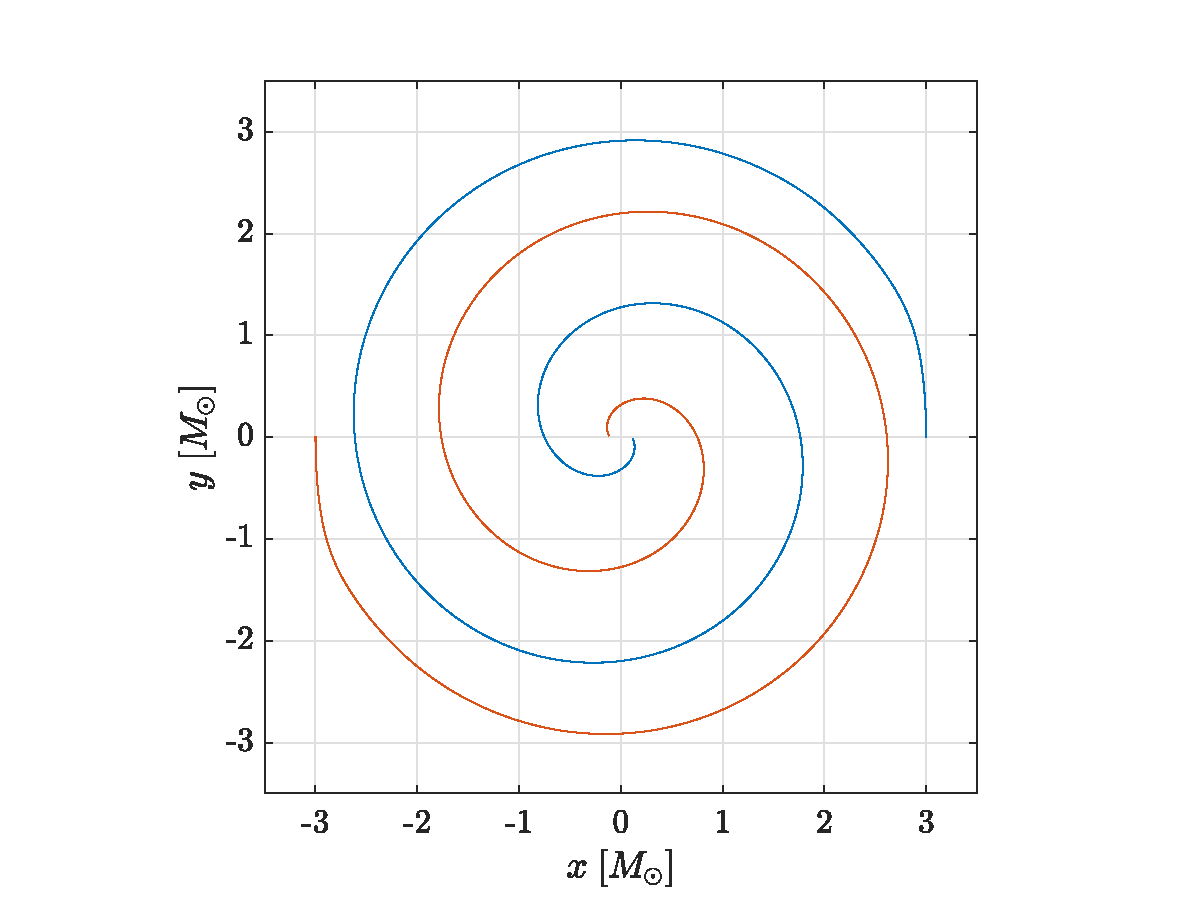
\includegraphics[width=.45\textwidth]{numerical_evolution/trajectory_b3.eps}
   \label{trajectory_b3}} \quad
   \subfloat[][Trajectory of the BBH with initial distance from the origin $b=4 \, M_{\odot}$.]
   {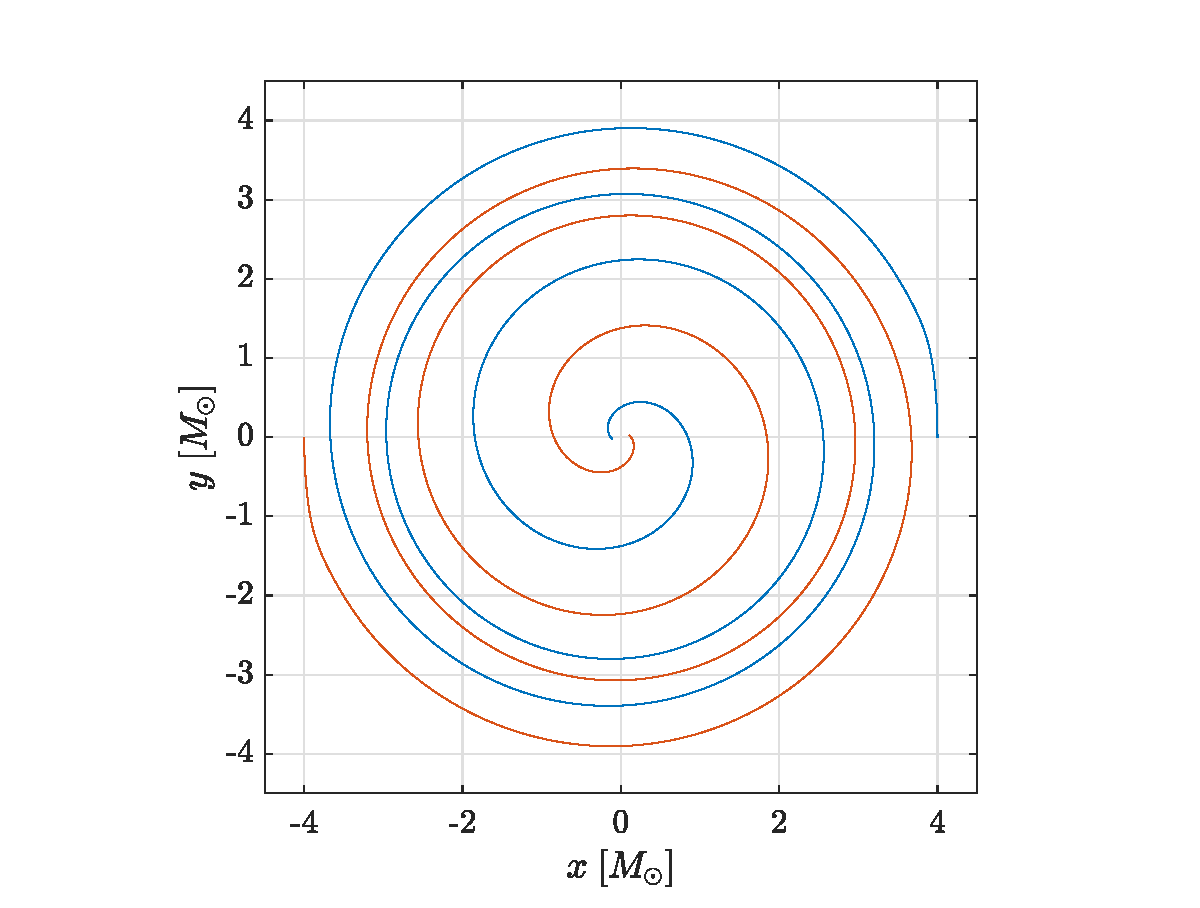
\includegraphics[width=.45\textwidth]{numerical_evolution/trajectory_b4.eps}
   \label{trajectory_b4}} \quad
\subfloat[][Trajectory of the BBH with initial distance from the origin $b=5 \, M_{\odot}$.]
   {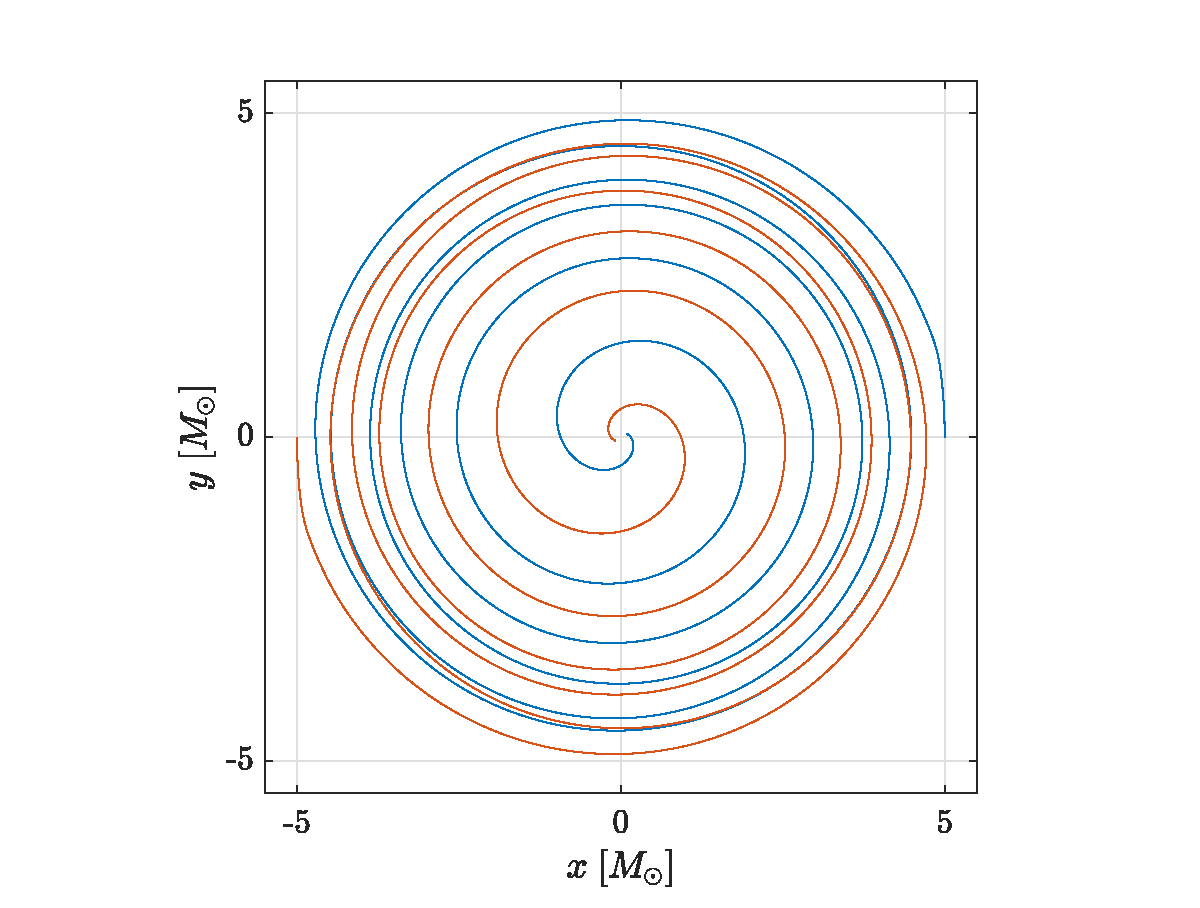
\includegraphics[width=.45\textwidth]{numerical_evolution/trajectory_b5.eps}
   \label{trajectory_b5}} \quad
\subfloat[][Trajectory of the BBH with initial distance from the origin $b=6 \, M_{\odot}$.]
   {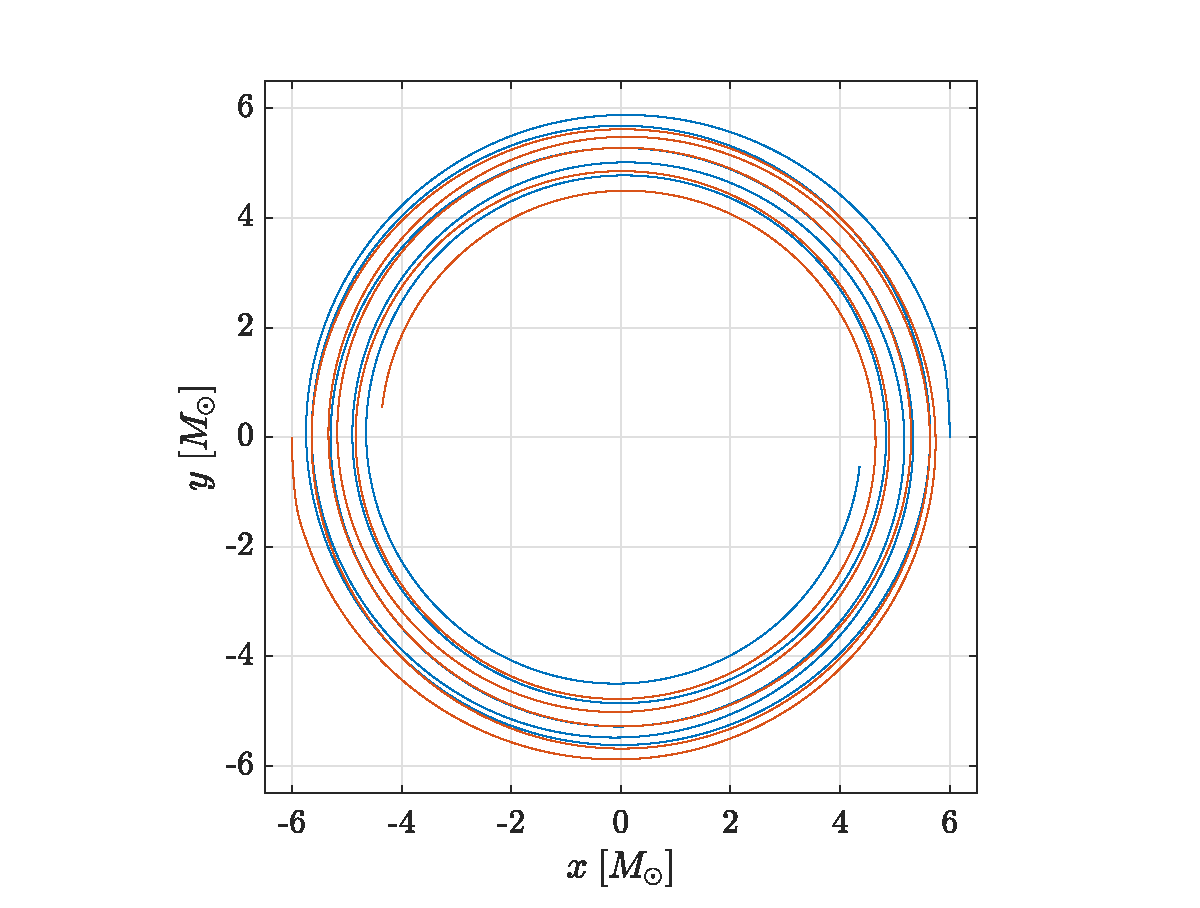
\includegraphics[width=.45\textwidth]{numerical_evolution/trajectory_b6.eps}
   \label{trajectory_b6}} \quad
\subfloat[][Trajectory of the BBH with initial distance from the origin $b=7 \, M_{\odot}$.]
   {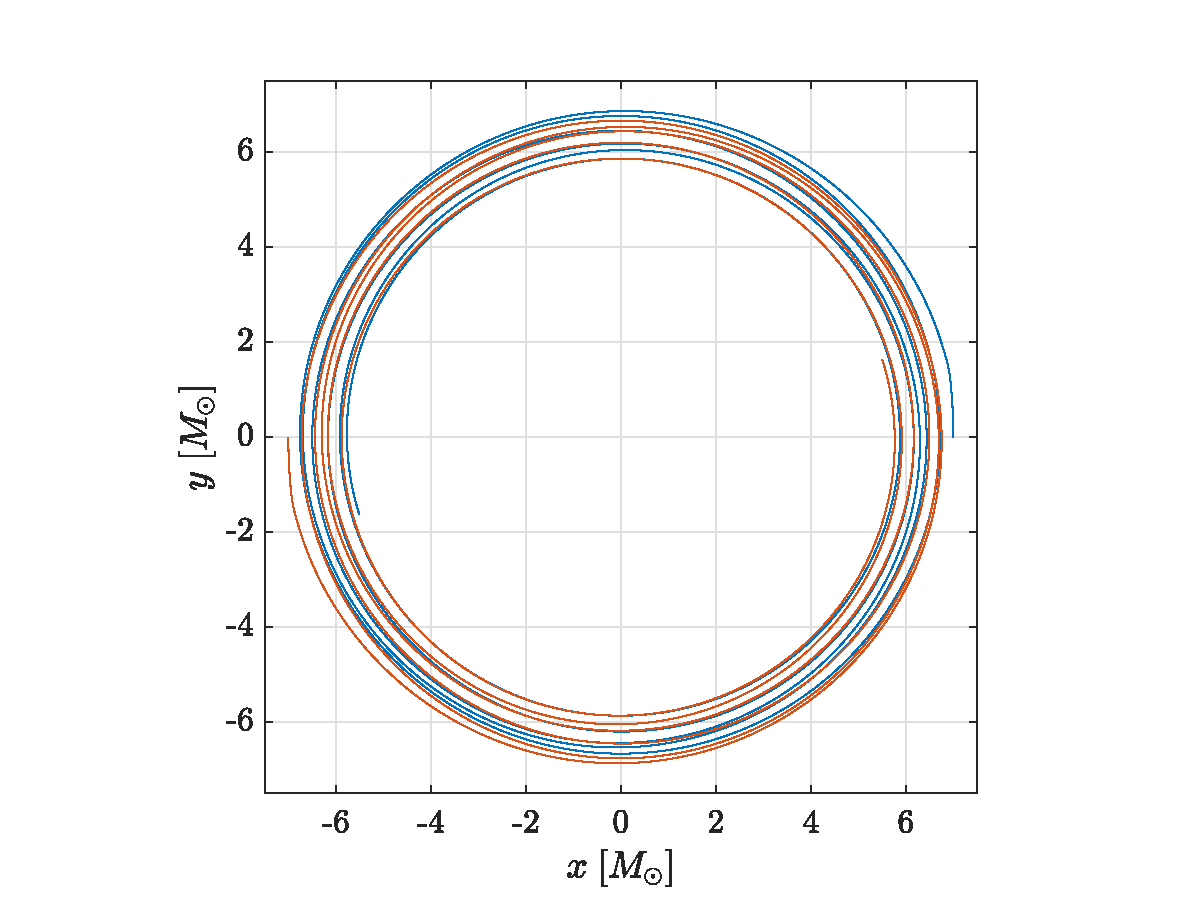
\includegraphics[width=.45\textwidth]{numerical_evolution/trajectory_b7.eps}
   \label{trajectory_b7}} \quad
\subfloat[][Trajectory of the BBH with initial distance from the origin $b=10 \, M_{\odot}$.]
   {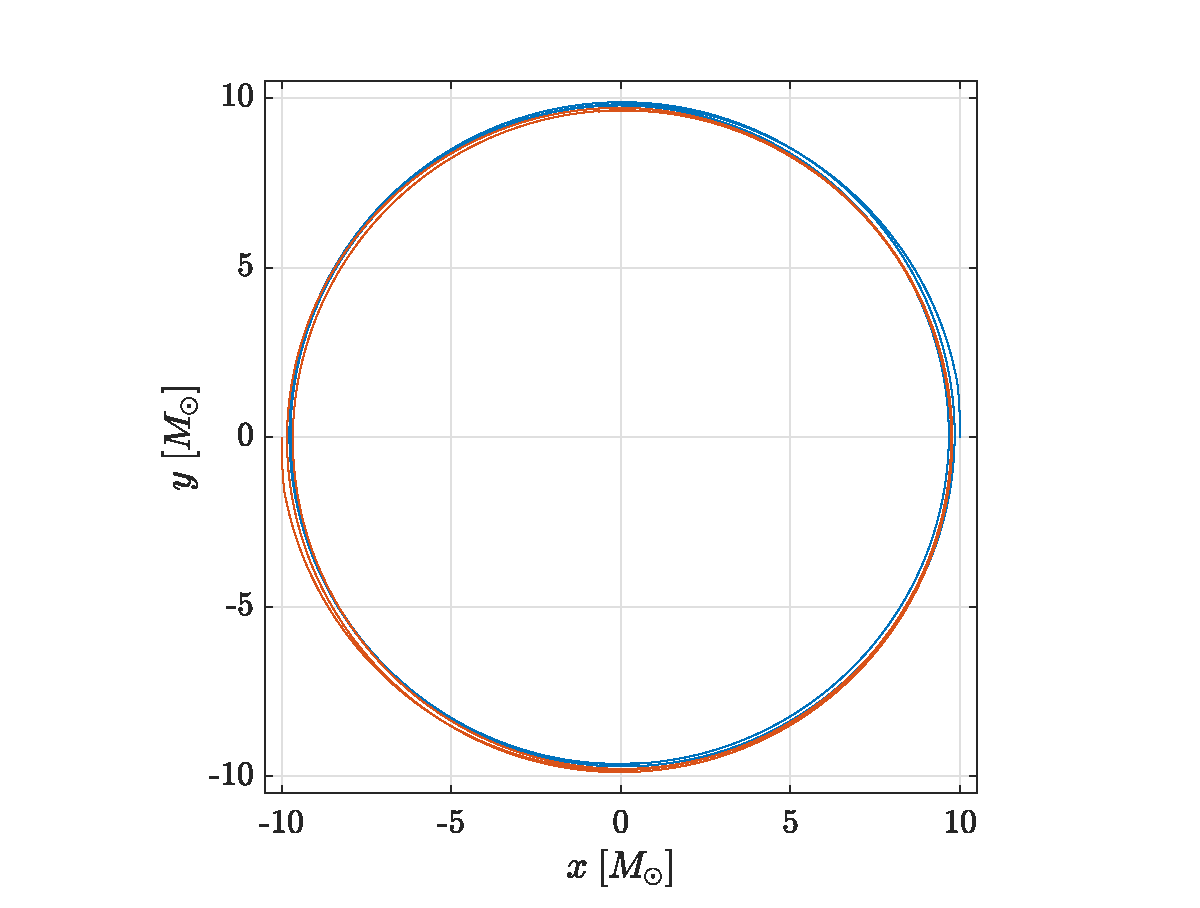
\includegraphics[width=.45\textwidth]{numerical_evolution/trajectory_b10.eps}
   \label{trajectory_b10}} \quad
 \\
\caption{It is shown the evolution of the BBH using the quasi-equilibrium initial conditions of Table(\ref{initial_conditions_bbh}). As the parameter $b$ increases, the orbits of the BBH tend to be more stable, where with stable we mean that the difference between the previous and the next orbit is small.}
\label{orbits}
\end{figure}
%%
%%
%%
%%
Due to the short initial distance from the origin, the BBHs with a  with low $b$ merge after few revolutions, for instance BBH-b3 merges after $2$ revolutions; BBH-b4 merges after
$3.5$ revolutions; BBH-b5 merges after $6$ revolutions.
Whereas the BBHs with an high parameter$b$ have orbits close to each other, such that they form a ring shape.\\
Notice that as the $b$ increases, the two black holes have orbits that drift apart from the coil-shaped path of Figure(\ref{trajectory_b3}).
This behavior can be better understood analyzing the distance of one of the balck hole from the origin as a function of time. 
For this reason, we plot in Figure(\ref{radius_evolution}) the normalized radial distance
\[
R(t)/b = \frac{\sqrt{x ^{2} (t) + y^{2} (t)}}{b}
\]
which depicts a new feature of the orbits. There are evident oscillations of the time-evolution of the radius $R(t)$.
%%
%%
%%
%%
\begin{figure}
\centering
    \textbf{Normalized Radial evolution of the BBH}\par\medskip
\makebox[\textwidth][c]{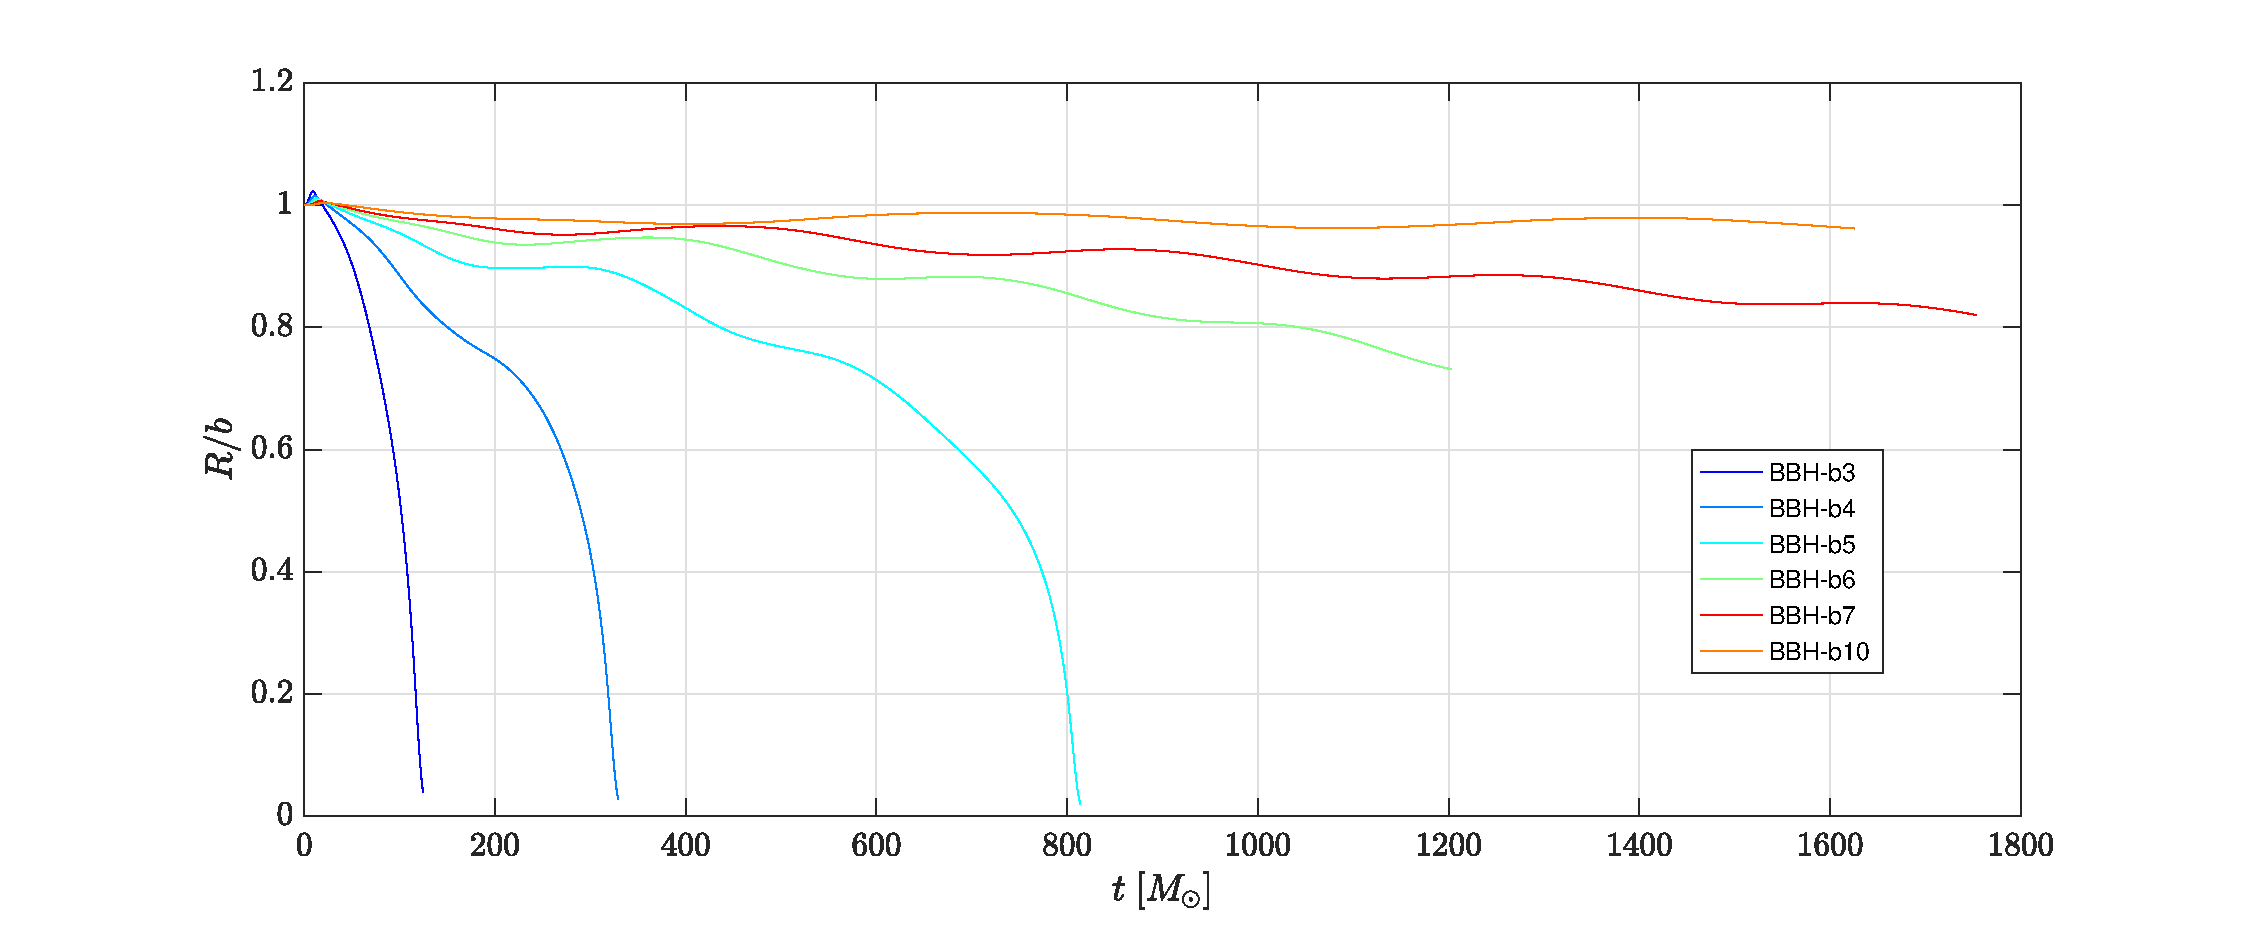
\includegraphics[width=1.1\textwidth]{numerical_evolution/radius_evolution.eps}}
\caption{Time evolution of the distance $R(t)$ between a black hole and the origin of the axes. The values are normalized to the initial separation from the origin $b$. The figure shows oscillation modes especially for BBHs with high $b$.}
\label{radius_evolution}
\end{figure}
%%
%%
%%
%%
\par
We now stufy the gravitational radiation emitted by the different binary sources is extracted following to the procedure described in section(\ref{gw_extraction}).\\
As we have seen in section(\ref{solution_linearized_einstein_eq}) the gravitational radiation scales with the distance from the source as $1/r$.
Therefore, in order to have an order of magnitude of the gravitational wave strain 
\[
h(t) = h_{+} - i h_{\times}
\] 
where $h_{+}$ and $h_{\times}$ are taken from equations(\ref{h_+_numerical}) and (\ref{h_x_numerical}), we multiply $h(t)$ by the distance at which it is was measured and we divide it by a typical cosmological distance of binary sources $r=100 \, \mega \text{pc} \approx 3.1 \times 10^{19} \, \kilo \meter$.
In addition, the units of time will be expressed in millisecond in order to easily compare the frequency of the signals with the sensitivities of the gravitational wave detetctors.\\
The gravitational singals are shown in Figure(\ref{gw_b3}), (\ref{gw_b4}), (\ref{gw_b5}), (\ref{gw_b6}), (\ref{gw_b7}) and (\ref{gw_b10}).
In the time interval $t \in (0,0.1)\milli \second$ the gravitational wave of all simulations $\psi_4$ shows an irregular perturbation. 
In [REF] it is pointed out that there is a numerical noise that could be reduced using a more refined simulations. However,   the simulations are enough accurate for our purpose after that time interval.\\ 
%%
%%
%%
%%
\begin{figure}[h]
\centering
    \textbf{Gravitational Wave emitted by BBH-b3}\par\medskip
\centering
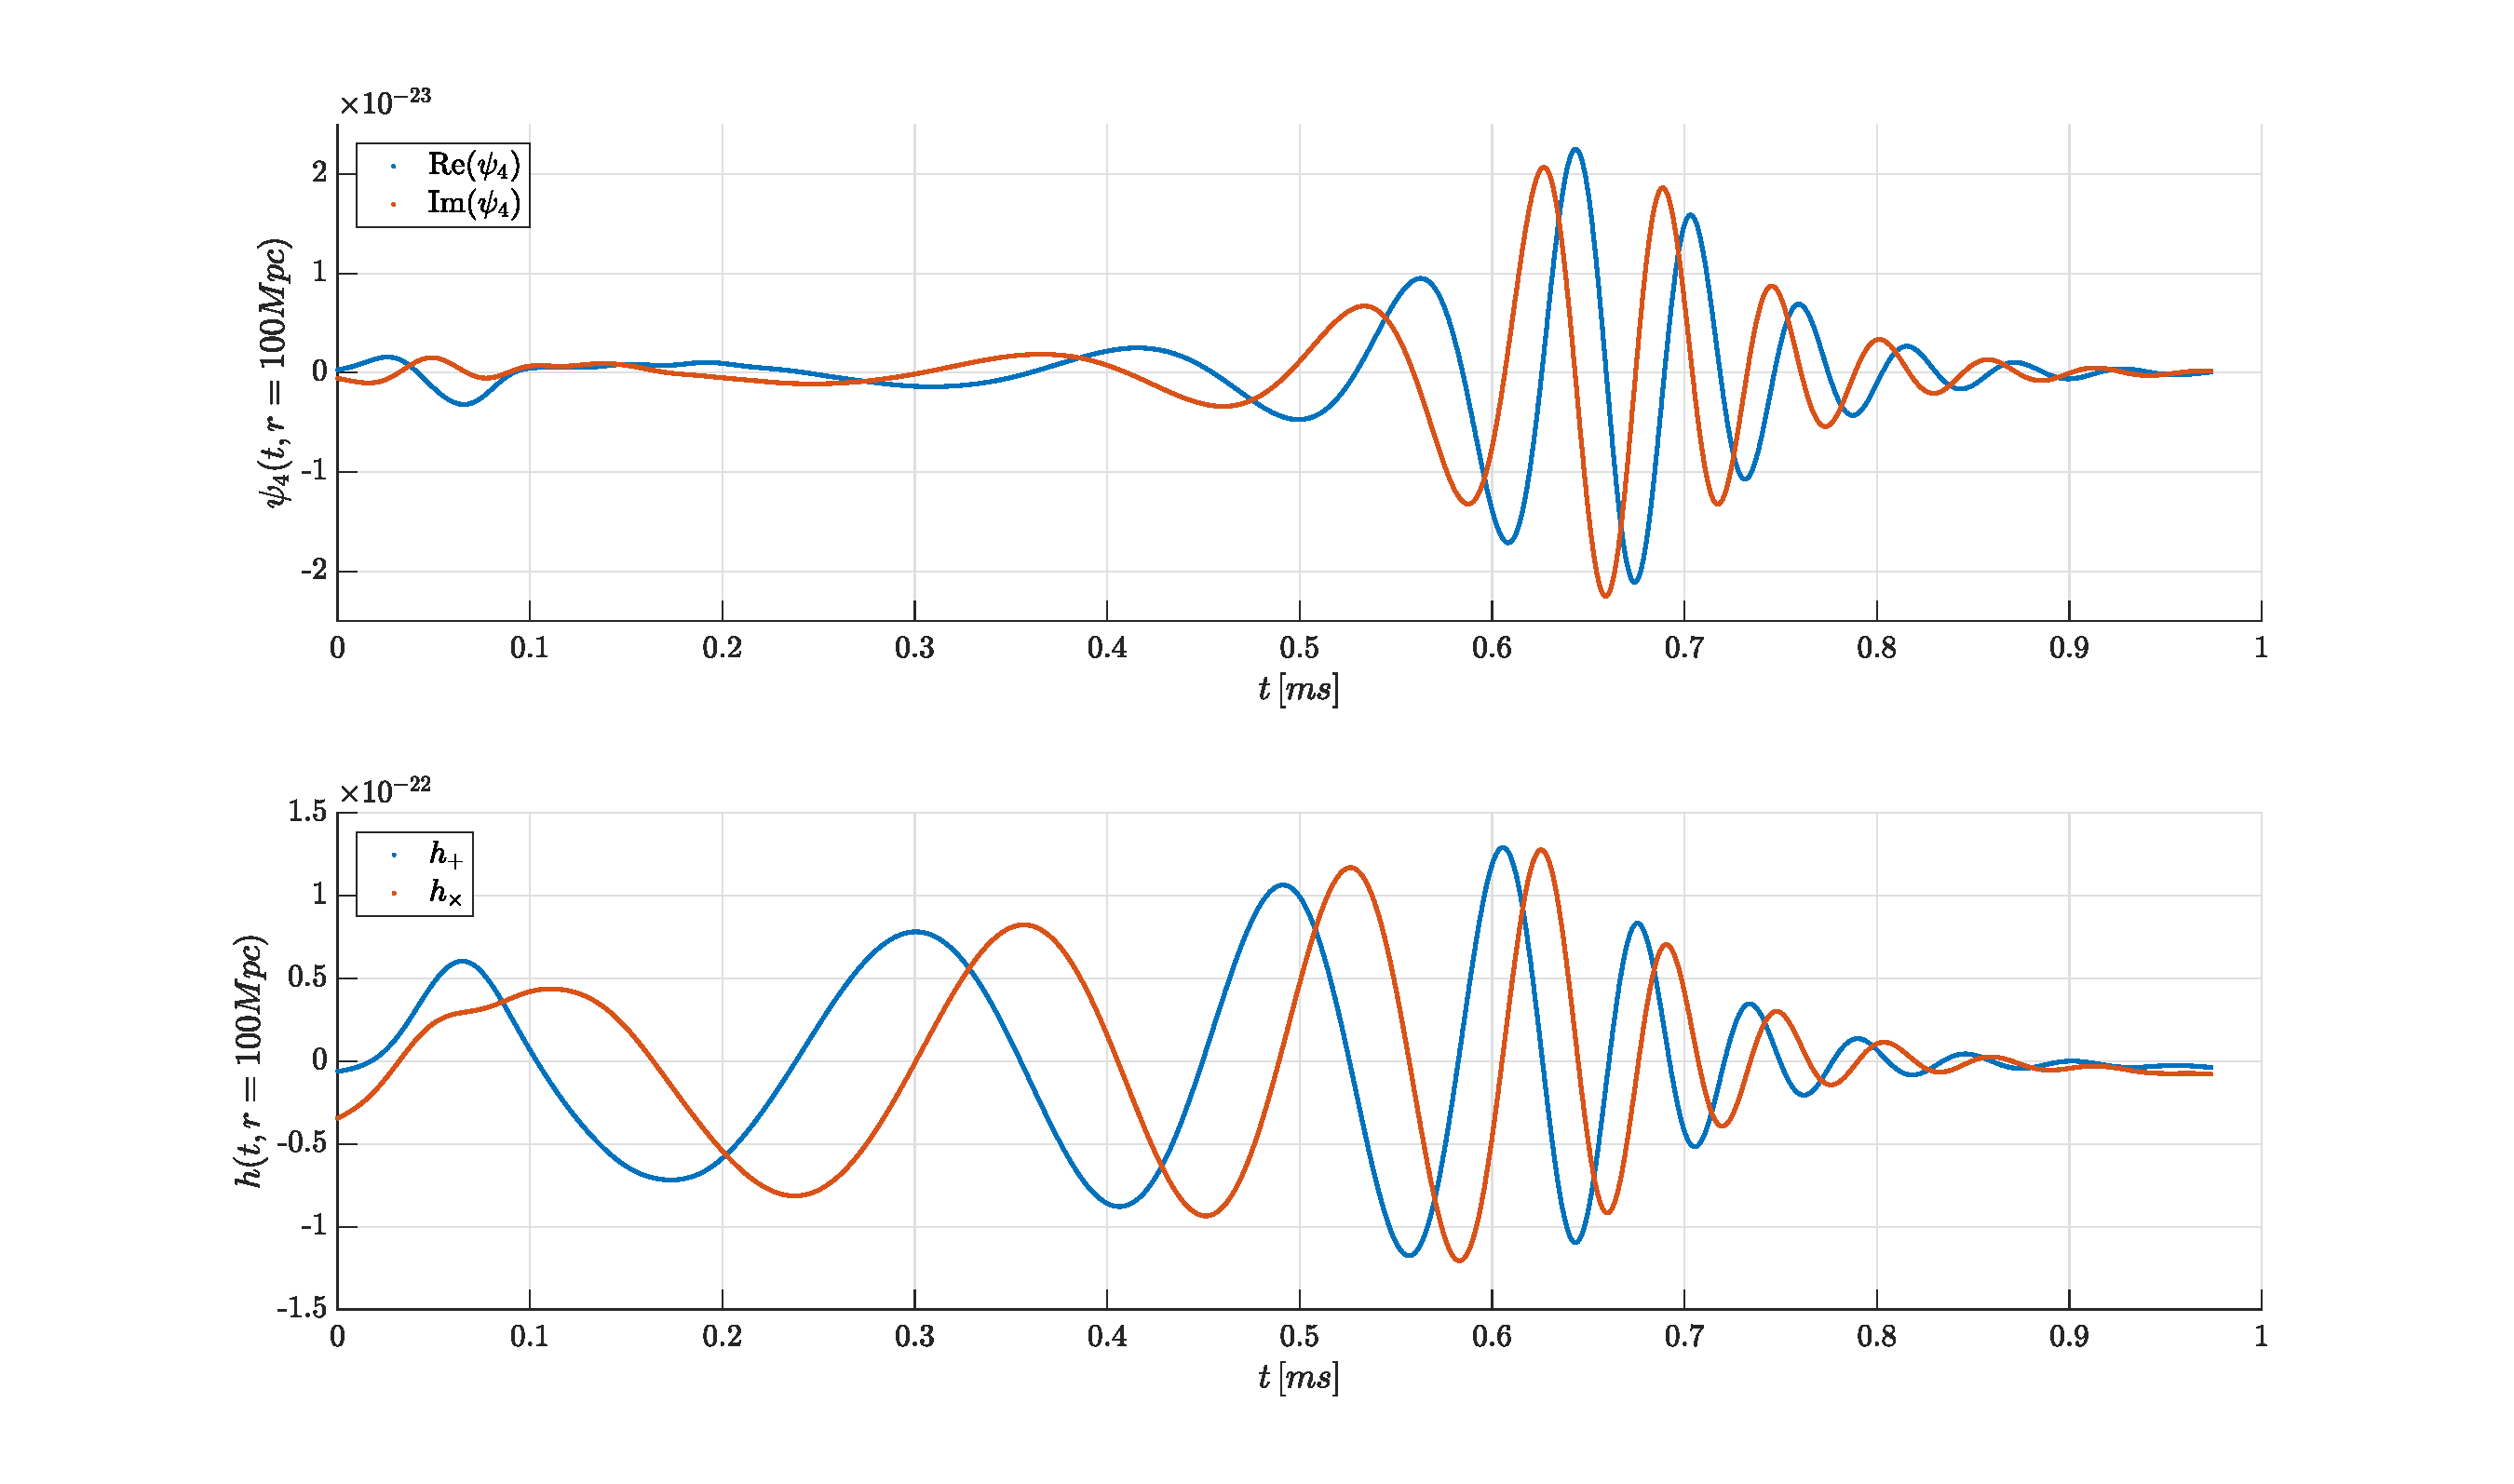
\includegraphics[width=1\textwidth]{numerical_evolution/gw_b3.eps}
\caption{The first and the second panels show, respectively the gravitational signal $\psi_4=\psi_4 ^{2,2}$ and the gravitational strain produced by the BBH-b3.}
   \label{gw_b3}
 \end{figure}
   %%
   %%
   %%
   %%
The GW radiated by the binary black hole with parameter $b=3$, in Figure(\ref{gw_b3}), has a short duration with respect to the others due to the intial conditions.
In fact, due to the strong interaction between the two bodies, the black holes merge quickly after $125 \, M_{\odot} \approx 0.616 \, \milli \second$ from Figure(\ref{radius_evolution}). 
The radius of the orbit decreases rapidly and the inspiralling phase lasts only $0.6 \milli \second$ and, as a consequence the waveform is a sinusoid with a noticeable varying frequency.
After $6.1 \milli \second$ the gravitational wave aplitude starts decreasing and oscillating around zero as expected in the ring-down phase, in which the black holes are already merged. 
\\
The gravitational radiations emitted of BBH-b4 and BBH-b5 are pretty similiar, they both show the typical phase of insipralling that can be approximated with a sinusoid analogue to the quadrupole formula.
   %%
   %%
   %%
   %%
\begin{figure}[h!]
\centering
    \textbf{Gravitational waves emitted by BBH-b4}\par\medskip
\centering
   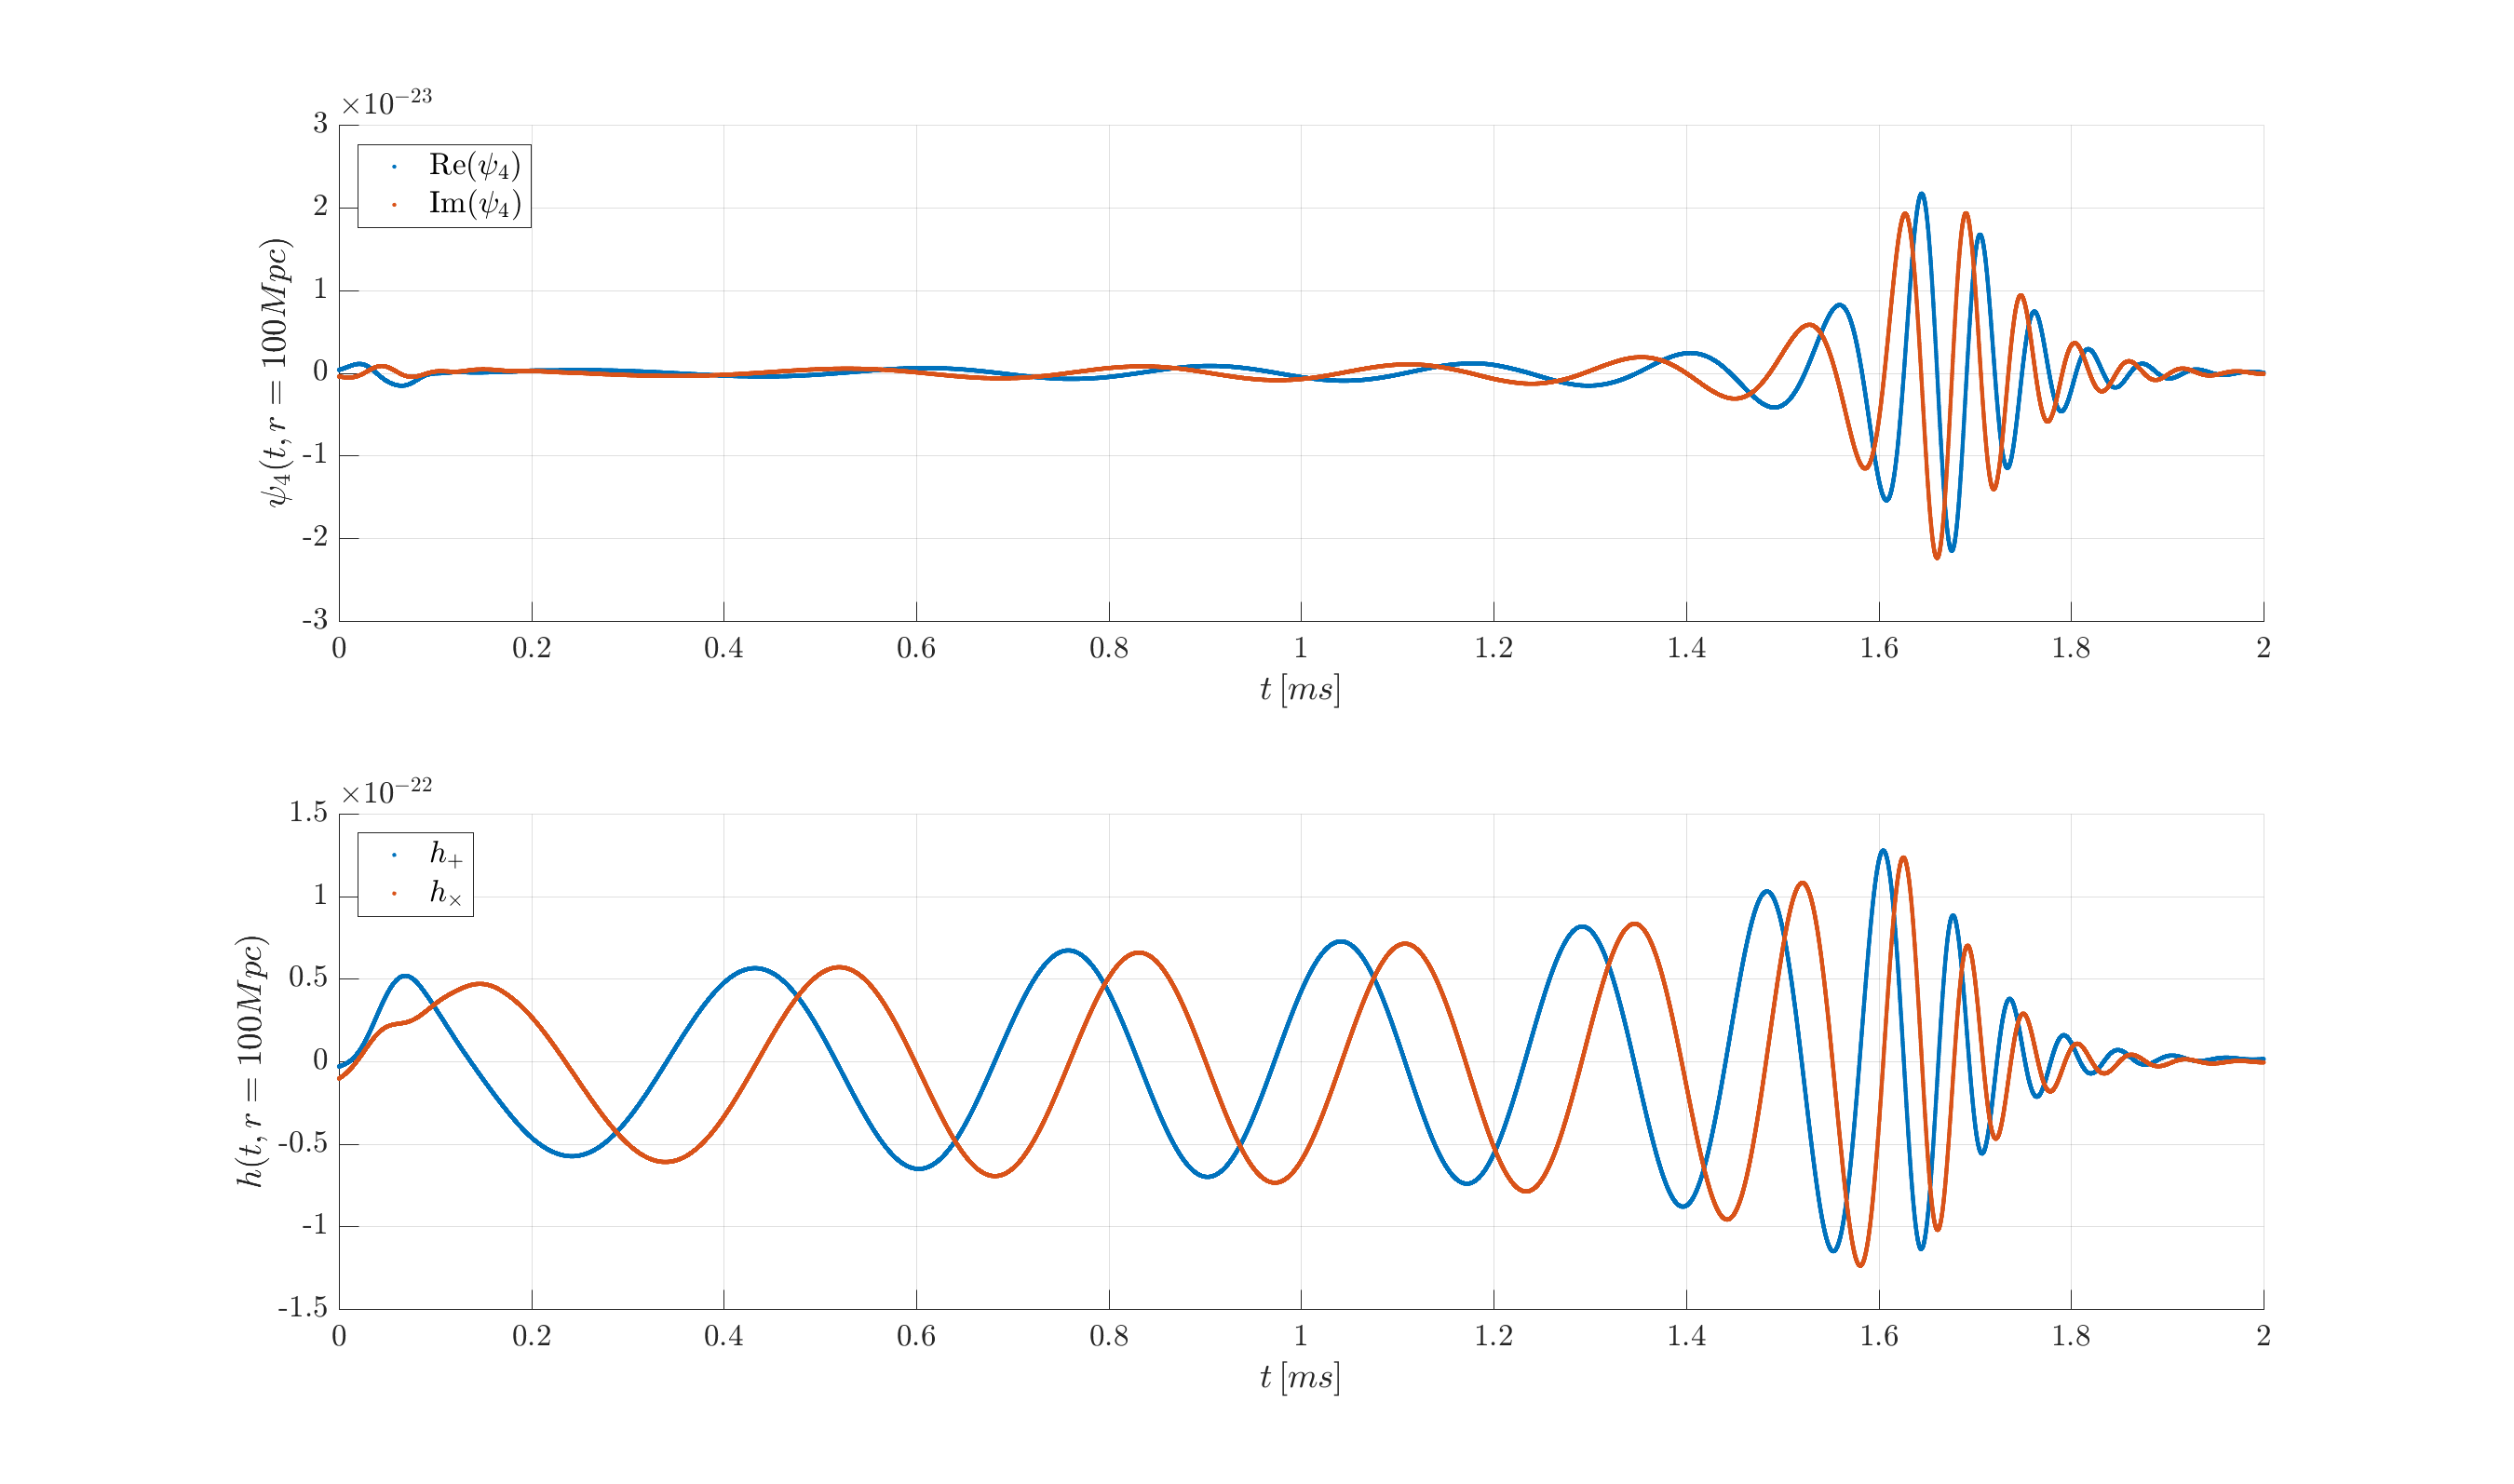
\includegraphics[width=1\textwidth]{numerical_evolution/gw_b4.eps}
   
   \caption{The first and the second panels show, respectively the gravitational signal $\psi_4=\psi_4 ^{2,2}$ and the gravitational strain produced by the BBH-b4.}
\label{gw_b4} 
\end{figure}
      %%
   %%
   %%
   %%
   \begin{figure}[h!]
\centering
    \textbf{Gravitational waves emitted by BBH-b5}\par\medskip
\centering
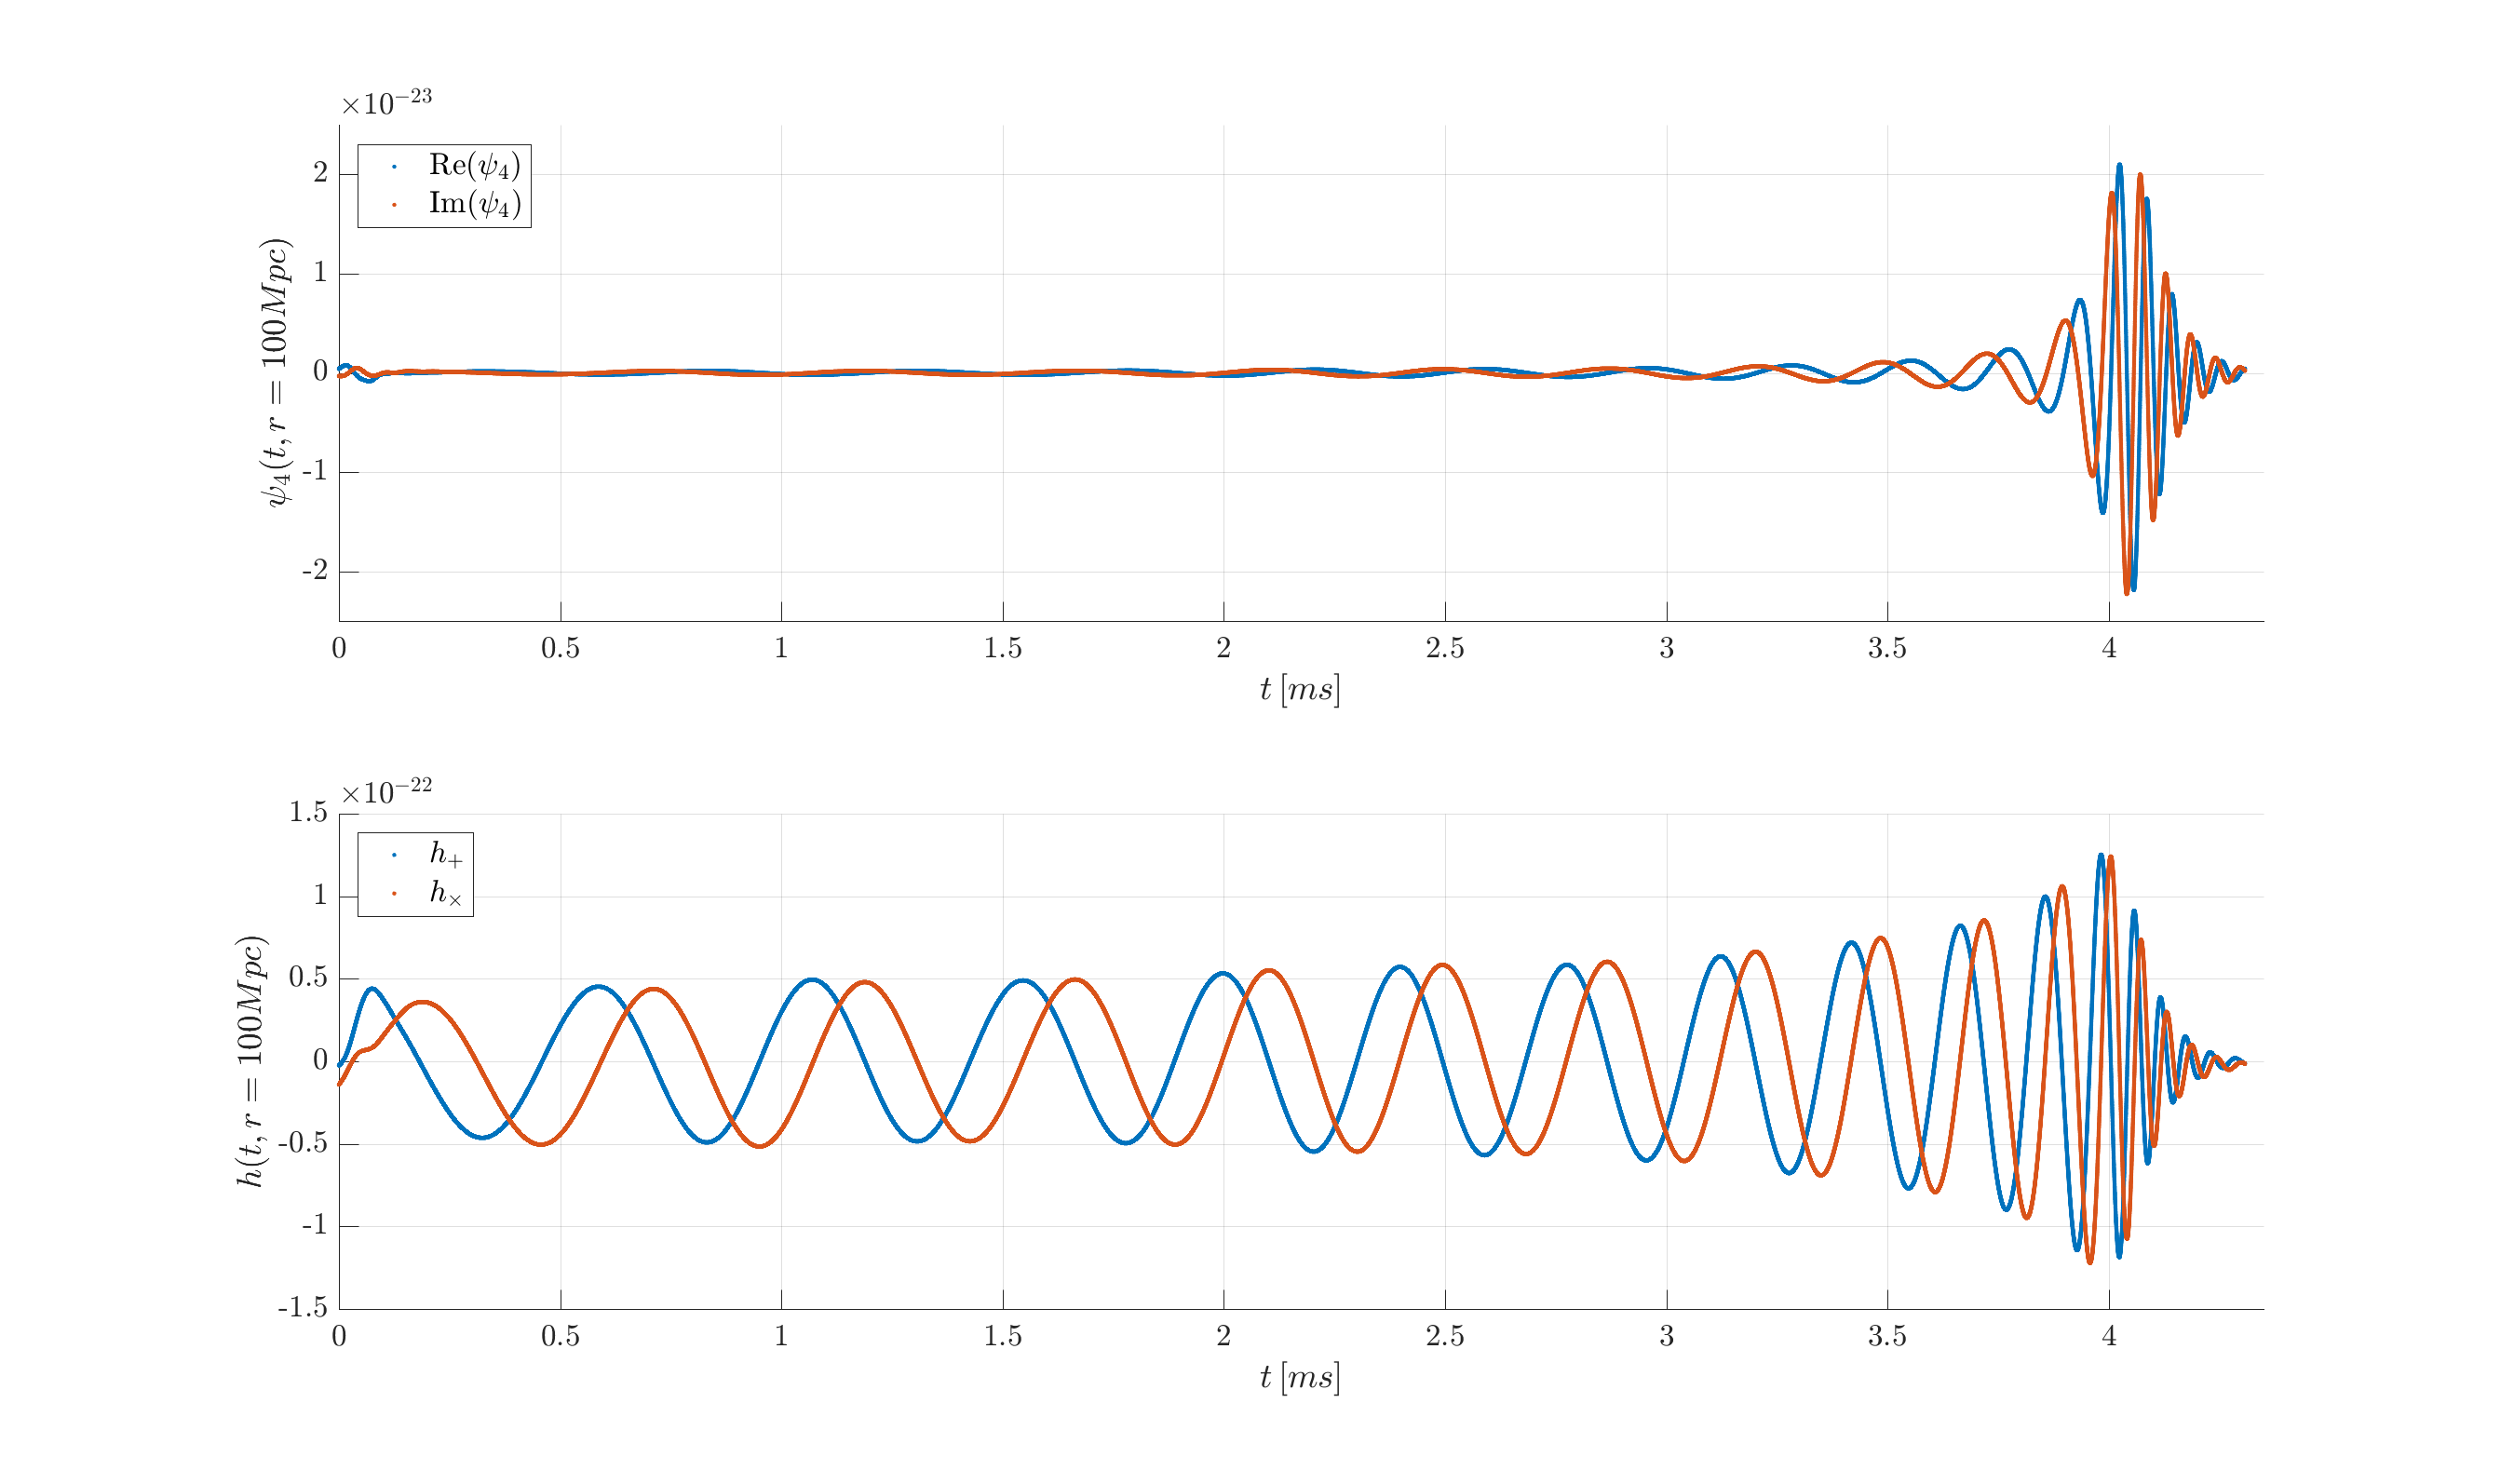
\includegraphics[width=1\textwidth]{numerical_evolution/gw_b5.eps}
   \caption{The first and the second panels show, respectively the gravitational signal $\psi_4=\psi_4 ^{2,2}$ and the gravitational strain produced by the BBH-b5.}
\label{gw_b5}
\end{figure}
   %%
   %%
   %%
   %%
Since the BBH-b5 has a initial configuration with further initial separation than BBH-b4, the signal of BBH-b5 lasts longer $4.5 \milli \second$ than the GW radiaition of BBH-b4 lasting $2 \milli \second$.\\
The gravitational strains $h$ of BBH-b3, BBH-b4 and BBH-b5 have similiar amplitudes, the strain increases its vale from $\approx 0.5 \times 10^{-22}$ up to $\approx1.5 \times 10^{-22}$ during the inspiralling, and the ring-doww phase lasts approximately $0.5 \, \milli \second$.\\
The gravitational signal $\psi_4$ radiated by the BBH-b6 source has big initial noise and it is affected by perturbations between $(1,1.5) \milli \second$. 
Alothough the gravitational strain $h$ will be affected by this perturbations, its oscillation modes in Figure(\ref{gw_b6}) are rather smooth. 
In a time interval of $5 \milli \second$ the amplitudes of the two polarizations $h_+$ and $h_{\times}$ vary, respectively, from $3.9\times 10^{-23}$ to $5\times 10^{-23}$, and from $3\times 10^{-23}$ up t $4.5\times 10^{-23}$. 
These small variations shows similiar features with the quadrupole formula approximation, which could roughly describe the inspiralling phase.\\
As expected, by increasing the parameter $b$, the gravitational strain decreases in intensity in the first part of the black hole evolution.\\
   %%
   %%
   %%
   %%
\begin{figure}
\centering
    \textbf{Gravitational waves emitted by BBH-b6}\par\medskip
\centering
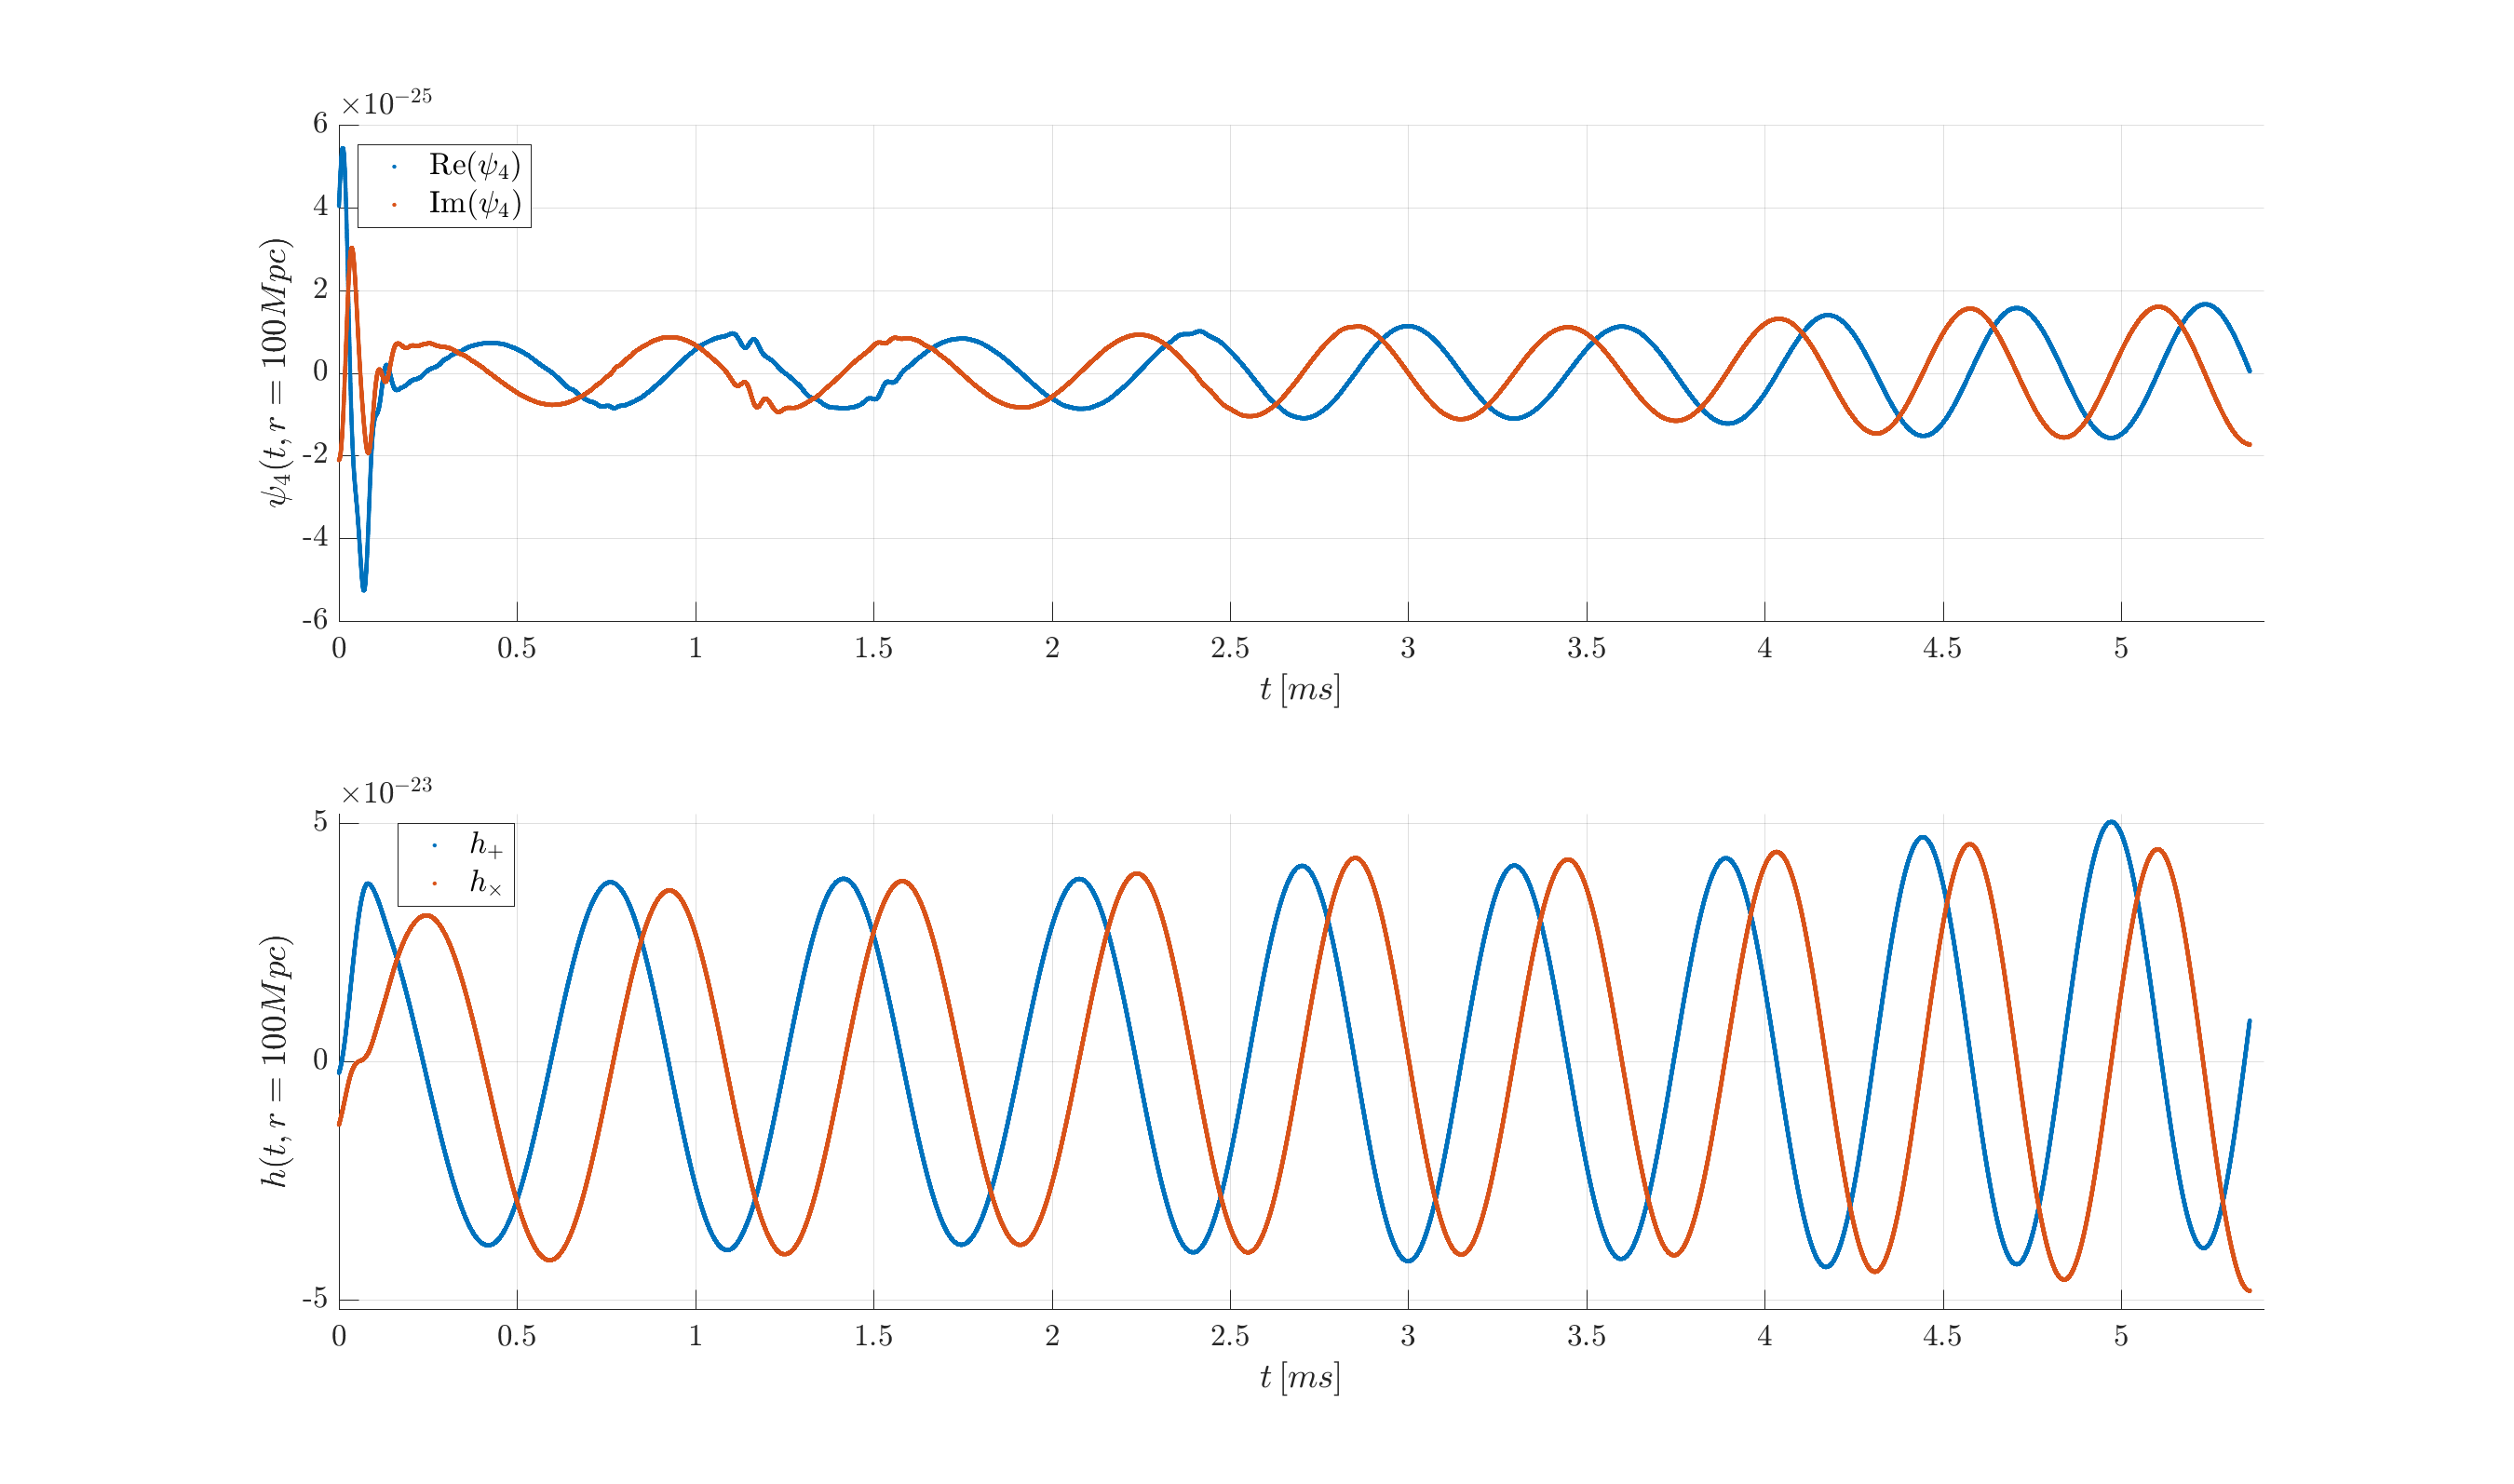
\includegraphics[width=0.9\textwidth]{numerical_evolution/gw_b6.eps}
   \caption{The first and the second panels show, respectively the gravitational signal $\psi_4=\psi_4 ^{2,2}$ and the gravitational strain produced by the BBH-b6.}
      \label{gw_b6}
\end{figure}
   %%
   %%
   %%
   %%
   \begin{figure}
\centering
    \textbf{Gravitational waves emitted by BBH-b7}\par\medskip
\centering
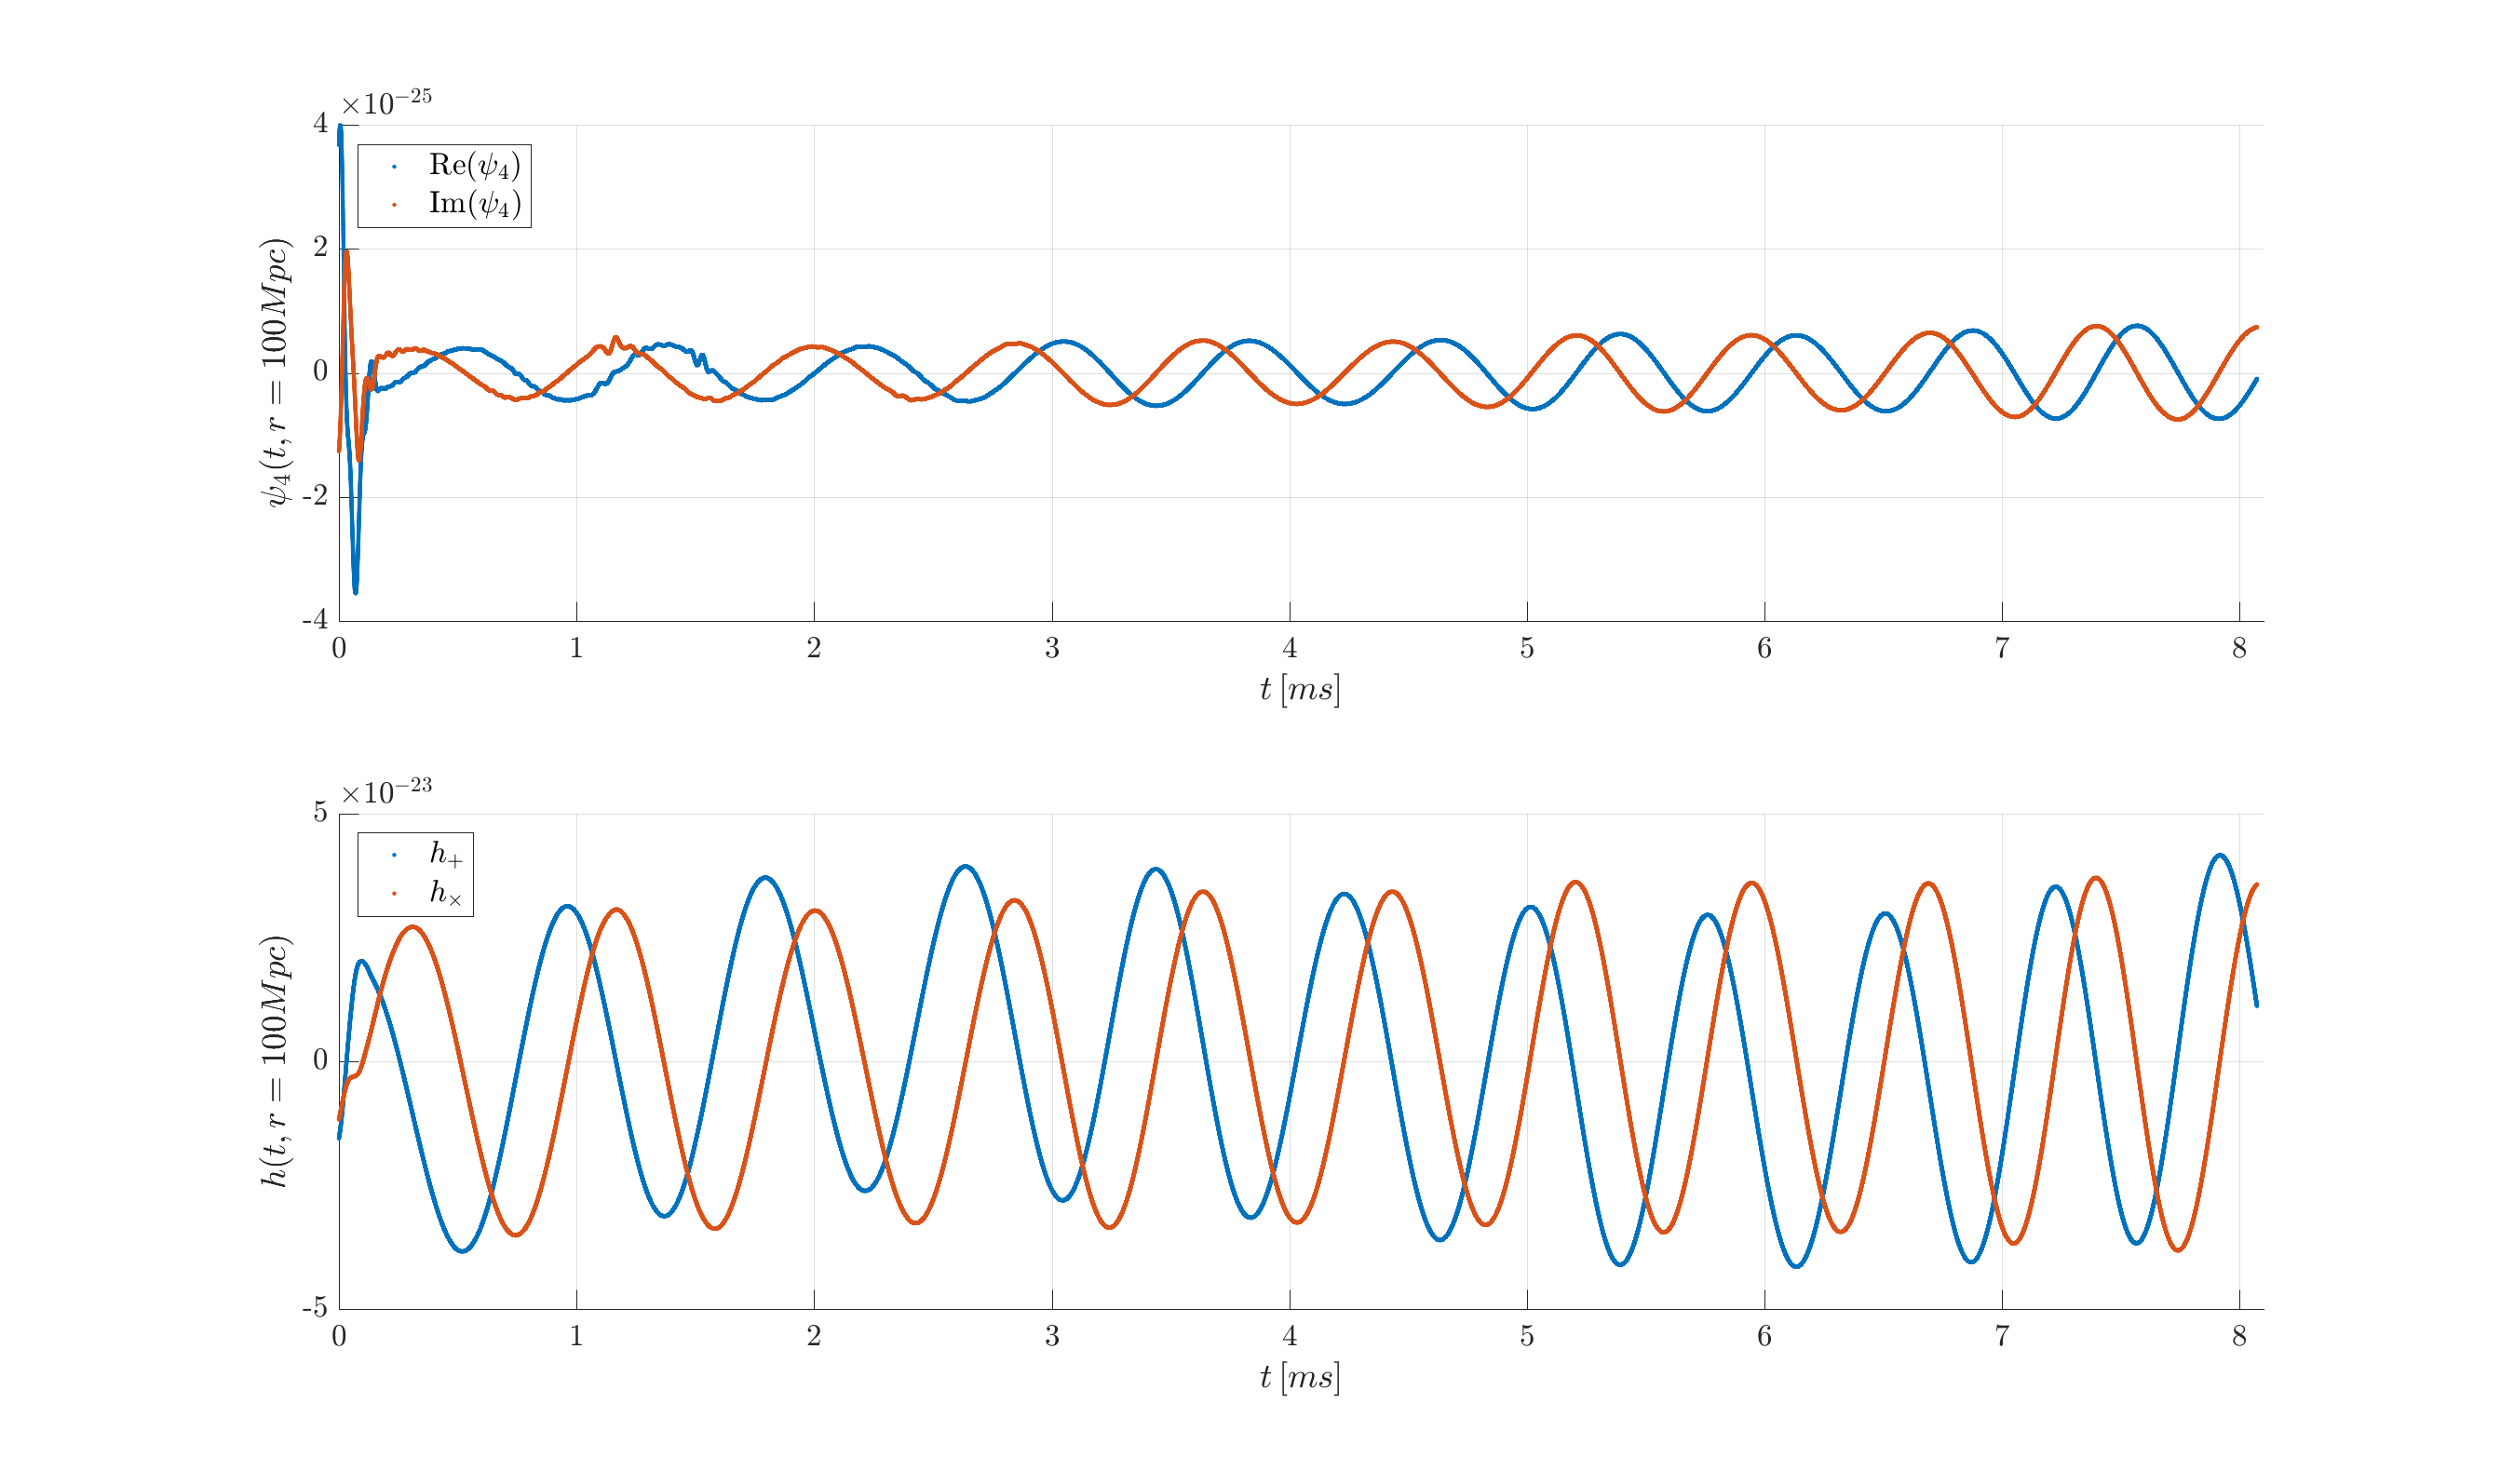
\includegraphics[width=0.9\textwidth]{numerical_evolution/gw_b7.eps}
\caption{The first and the second panels show, respectively the gravitational signal $\psi_4=\psi_4 ^{2,2}$ and the gravitational strain produced by the BBH-b7.}   
   \label{gw_b7}
   \end{figure}
   %%
   %%
   %%
   %%
      \begin{figure}
\centering
    \textbf{Gravitational waves emitted by BBH-b10}\par\medskip
\centering   
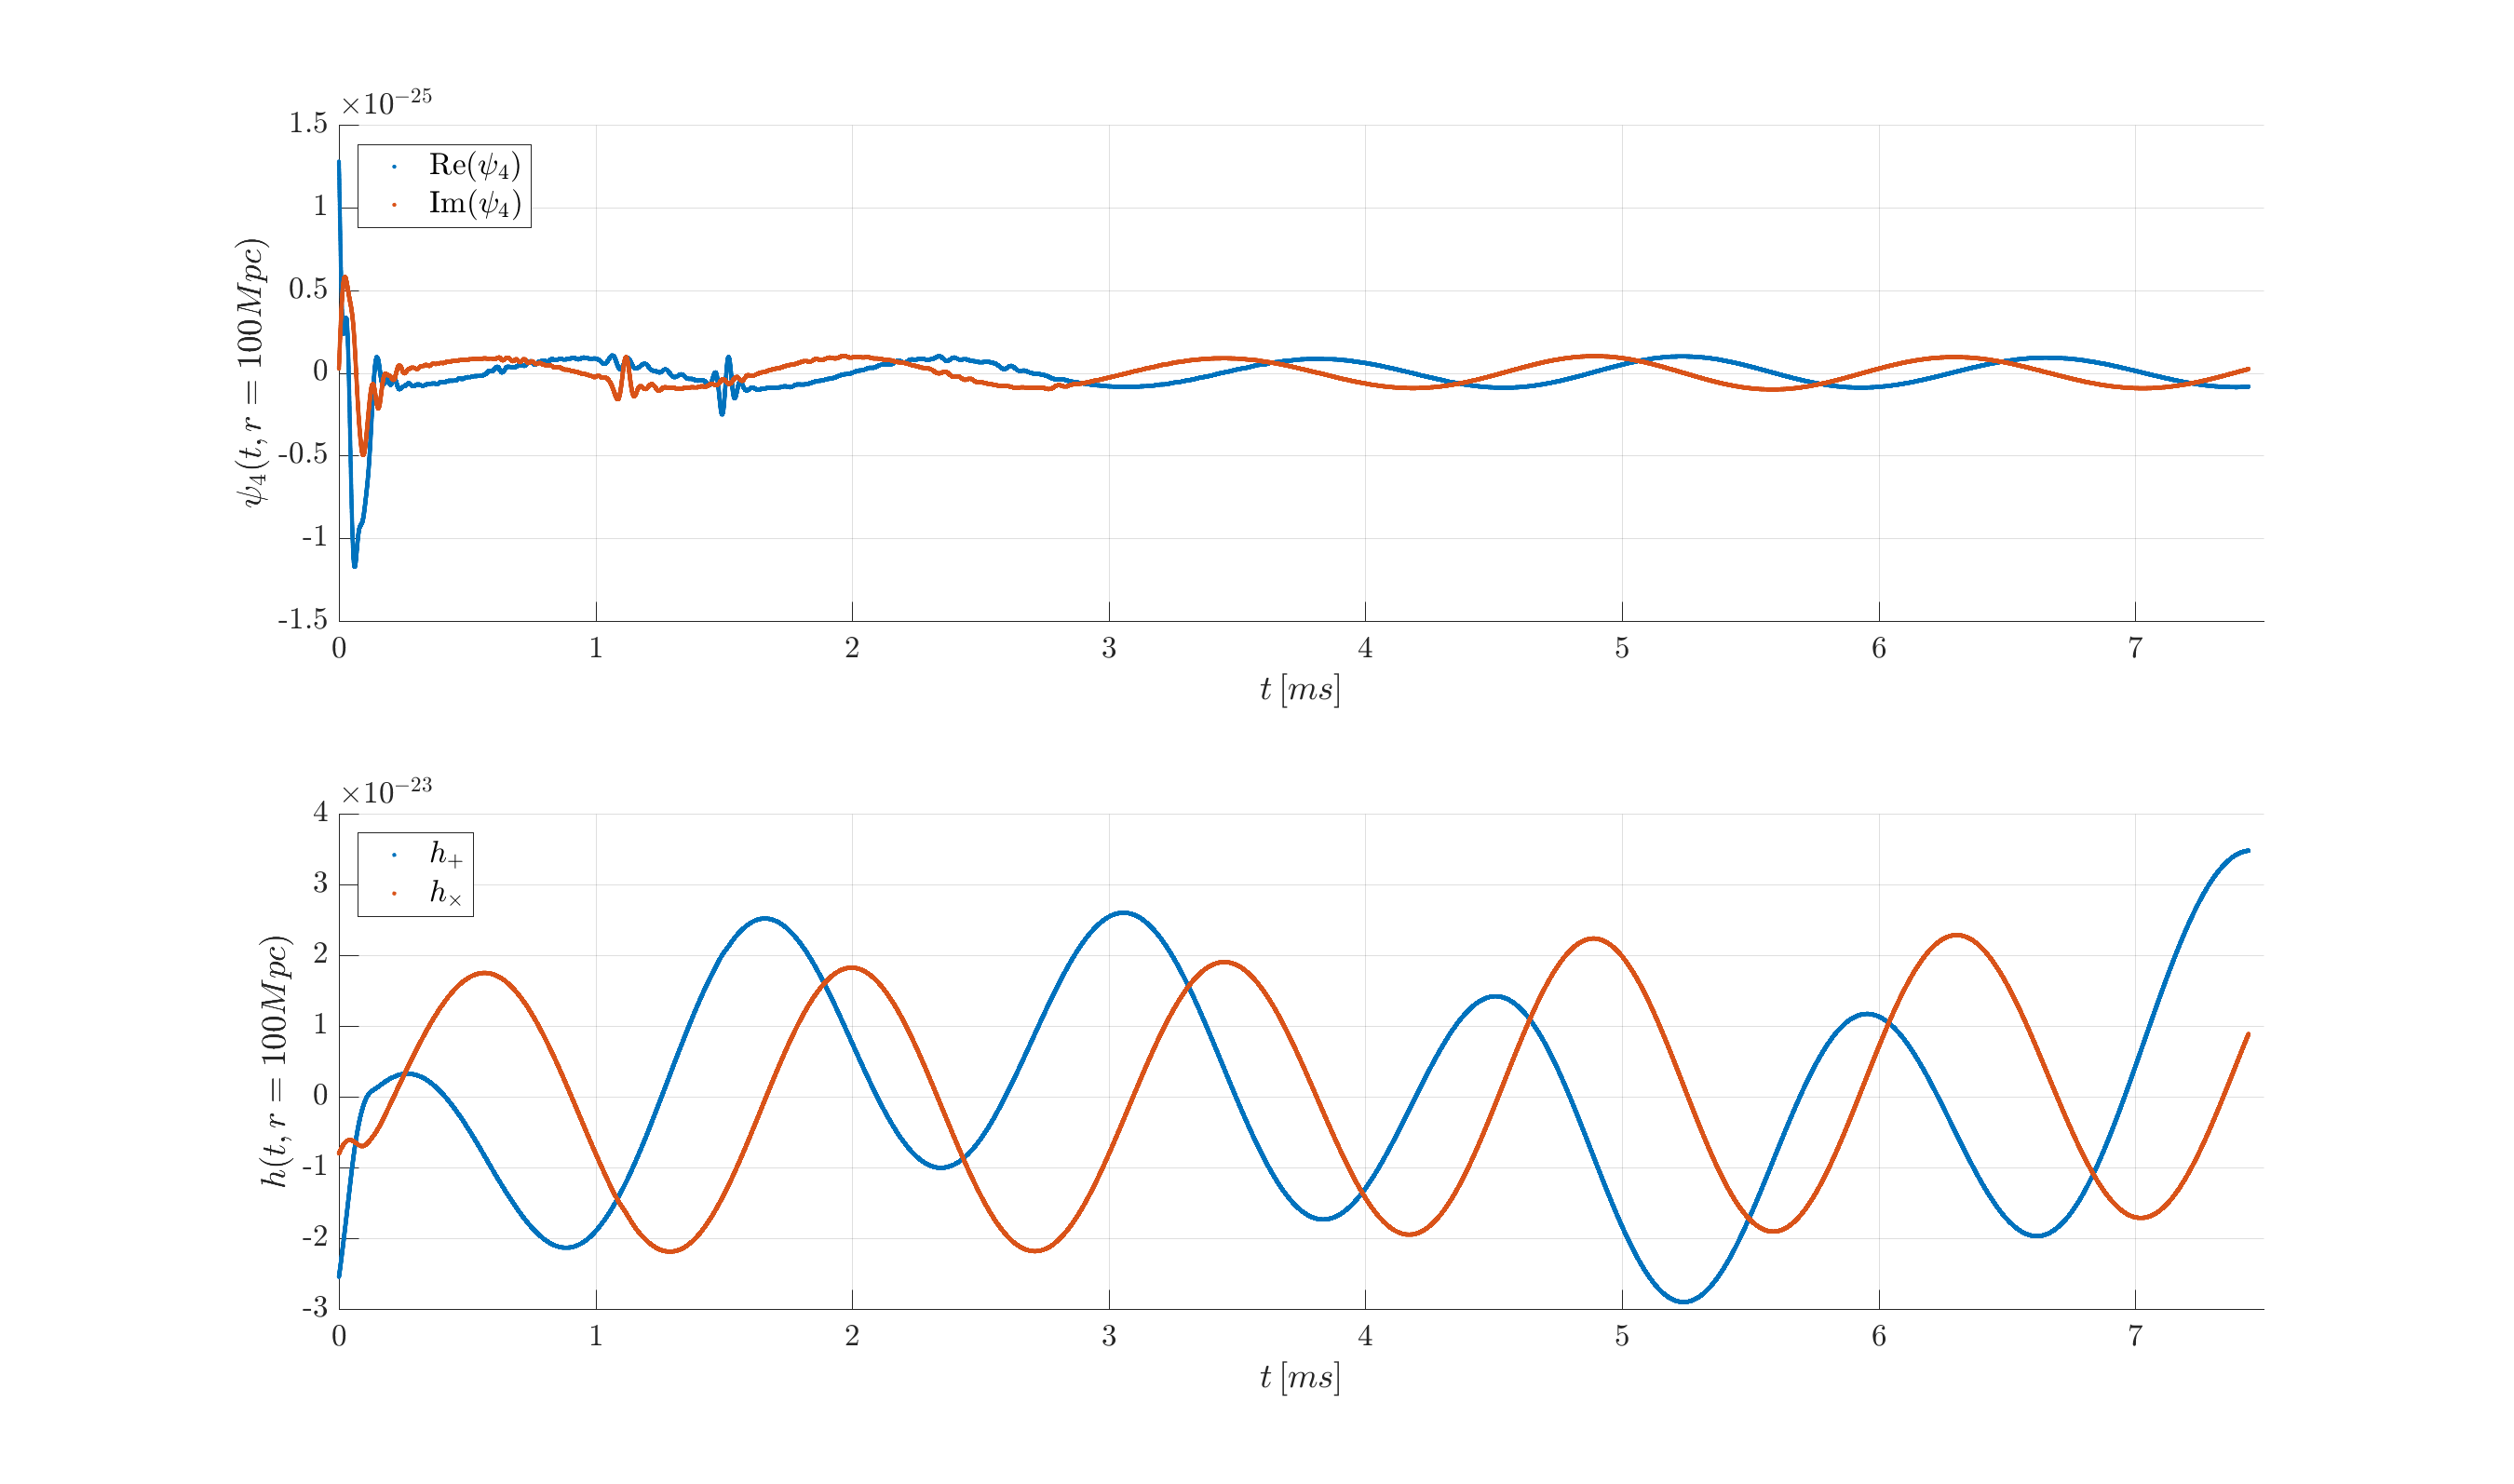
\includegraphics[width=0.9\textwidth]{numerical_evolution/gw_b10.eps}
\caption{The first and the second panels show, respectively the gravitational signal $\psi_4=\psi_4 ^{2,2}$ and the gravitational strain produced by the BBH-b10.}
\label{gw_b10}
\end{figure}
%%
%%
%%
%%
The $\psi_4$ signals produced by BBH-b7 and BBH-b10 have noises analogue to those of BBH-b6, however they manifest  a new feature in the gravitational strain $h$.
Indeed, it is evident from Figures (\ref{gw_b10}) and (\ref{gw_b7}) that the two polarization $h_{+}$ and $h_{\times}$ have another oscillation mode with larger period that the typical sinusoidal oscillation mode.\\
The consequence of such behavior could be due to a rough numerical exctraction, or to the oscillations in the radial distance from the center in Figure(\ref{radius_evolution}).\\
As a matter of fact, the waveform that can be better approximated using our rudimentary methods of analysis is that on of BBH-b6.\\
An important result obtained through the quadrupole formula applied to a binary source was that the frequency of the gravitational wave is twice the orbital frequency of rotating bodies.
Using the Fourier transform of the gravitational strain and the angular frequency data of the black holes we can test this hypothesis.







FEATURES OF ALL OF THEM
PHASE OF THE REAL AND OF THE IMAG


\subsection{Binary Neutron Star}